%%%%%%%%%%%%%%%%%%%%%%%%%%%%%%%%%%%%%%%%%%%%%%%%%%%%%%%%%%%%%%%%%%%%%%
%%% $LastChangedDate: 2022-04-19 19:09:28 +0200 (Di, 19 Apr 2022) $ (local)
%%% $LastChangedRevision: 2666 $
%%% $LastChangedBy: lf1agure $
%%% $Id: programmermanual.tex 2666 2022-04-19 17:09:28Z lf1agure $
%%%%%%%%%%%%%%%%%%%%%%%%%%%%%%%%%%%%%%%%%%%%%%%%%%%%%%%%%%%%%%%%%%%%%%
% Assumptions:
% * \ifPublicRelease is false throughout the compilation of this
%   document.

\documentclass[11pt,a4paper,twoside]{article}

\def\DocumentationType{Programmer's Manual}

% Authors:
\author{%
\ProjectAdministrator\thanks{\ProjectAdministratorsFootnoteText},
%
Alexander Weber,
Hao Zhou
}

% Abstract:
\def\AbstractText{%
\ProjectAcronym{} is a software to solve synthesis, analysis and
verification problems for infinite state dynamical systems.
This document provides information useful for programmers as well as
for expert users.
Readers are assumed to be familiar with the companion document
\cite{ABS_UsersManual}, with the \texttt{bash} shell script language
\cite{GNUbashManual}, and with the programming languages C
\cite{KernighanRitchie88} and Ada \cite{Barnes14} and the various
related development tools. Experience with the tools \texttt{make}
\cite{GNUmakeManual} and \texttt{svn} \cite{svnManual11} is an
advantage.
A computer running Linux should be used.
}

\usepackage{utils/main}

\svnid{$Id: programmermanual.tex 2666 2022-04-19 17:09:28Z lf1agure $}

\RequirePackage{tikz}
\usetikzlibrary{arrows}

\begin{document}
\maketitle\cleardoublepage\tableofcontents\cleardoublepage

\section{Quick Start}
\label{s:QuickStart}

\ProjectAcronym{} is a software to solve synthesis, analysis and
verification problems for infinite state dynamical systems.
Follow the steps below
to quickly get a copy of \ProjectAcronym{} running on your computer,
and to see it applied to an example.

\paragraph{Prerequisites.}
\ProjectAcronym{} is an implementation
of the symbolic controller synthesis framework
introduced in \cite{ReissigWeberRungger17} and
has been presented in \cite{WeberMacoveiciucReissig22}.
Users are assumed to be familiar with both of the aforementioned
documents.

\ProjectAcronym{} should be run on Linux,
which is what we assume throughout this document.
Some external software is required as well;
we recommend to proceed with the following steps and
follow the instructions printed out on the screen.
If this does not work, please refer to
Section \ref{s:SystemPrerequisites}
for more specific requirements.

We also assume that you are a
member of the project administrator's group at the
\ProjectHostInstitution{}. Otherwise, please refer to
\cite[Section ``Quick Start'']{ABS_UsersManual}
for ways to obtain (read) access to the latest public
version of \ProjectAcronym{}.

\ProjectAcronym{} is maintained using the version control system
\verb|svn| \cite{svnManual11}, and access is by user
name and password.

If you have an active account with the Central Computing Facilities
at the \ProjectHostInstitution{}, then you may use the user name
(``RZ-Kennung'') and password of that account. You should ask the
project administrator via email for access to
the \ProjectAcronym{} repository, providing your full name and your
user name.

Otherwise, choose user name and password on your own, where the former
should be of the form
\nolinebreak{$<$last name with capital initial$>$\verb|_|$<$capital
first name initial(s)$>$.} Then create an encrypted authentication
record, providing your password on request:
\begin{flushleft}
\verb|>| \verb|htpasswd -n | $<$user name$>$
\end{flushleft}
If the user name is \verb|Euler_L|, the output of the
command will be similar to
\begin{flushleft}
\verb|Euler_L:$apr1$y0Udv6R3$AgaYrEUkaLm85Cy/wcsmb0|
\end{flushleft}
and should be included in your email to the project administrator.

\paragraph{Obtaining a copy of \ProjectAcronym.}
Create a working copy of \ProjectAcronym{} in a local directory of
your choice, which may take some time:
\begin{flushleft}
\verb|>| \verb|svn checkout --username |
$<$user name$>$ \verb|\|\\
\verb|>| \expandafter\verb\expandafter|\RootAddressOfProjectInRepository |
$<$full path to working copy of \ProjectAcronym{}$>$
\end{flushleft}

\paragraph{Solving a simple synthesis problem.}
Please proceed as in \cite[Section ``Quick Start'']{ABS_UsersManual}.

\section{System Prerequisites}
\label{s:SystemPrerequisites}

\subsection*{Computing Platforms}
%\label{s:SystemPrerequisites:Platforms}

\ProjectAcronym{} is designed to solve synthesis, analysis and
verification problems on platforms represented by any of the target
triples listed in \ref{tab:RemoteMachines}. For more details, see
Sections \ref{s:organization:Structure:TopLevelBuild} and
\ref{s:organization:Structure:Platforms}.
%
\begin{table}[th]
\centering
{
\renewcommand{\arraystretch}{1.1}%
\tabcolsep1.5pt%
\begin{tabularx}{\linewidth}{l|l|l|l|X}
& \multicolumn{3}{c|}{Example Host Computer} &
\\
Platform Target Triple & Name & IP & CPU & Restrictions
\\
\hline 
\verb|x86_64-linux-gnu|\footnotemark &
 &
 &

&
--
\\
\verb|x86_64-suse-linux| &
 &
 &
 &
--
\end{tabularx}
}
\caption{\label{tab:RemoteMachines}%
Platforms on which \ProjectAcronym{} can be used.
}
\end{table}
\footnotetext{Synonym for \nolinkurl{x86_64-pc-linux-gnu}.}
%
Make sure that standard tools such as
\verb|make|, the \verb|bash| shell and \verb|gcc|
are available.
You may run \verb|gcc -dumpmachine| to check the target triple
representing your system.

\subsection*{AdaCore GNAT GPL and the GNAT Academic Program}
%\label{s:SystemPrerequisites:GNAT_GPL}

The software collection AdaCore GNAT GPL (see \url{https://www.adacore.com/})
facilitates building and using \ProjectAcronym{} on those platforms
for which no restrictions are given in \ref{tab:RemoteMachines}.
Its 2016 version is included in
the repository as a \verb|tar.gz| file which will be automatically
extracted once before the very first computation. Some support for
this software collection can be obtained using our subscription to the
GNAT Academic Program (GAP):
\begin{verbatim}
Account 2112: UNI BW MUNCHEN
GNAT Academic Program
\end{verbatim}
Access via GNATtracker, \url{www.adacore.com/academia}, using your
email address and your password. Requires registration.

% \subsection*{GNAT Pro Enterprise Subscription}
% %\label{s:SystemPrerequisites:GNAT_Pro}
% % possible improvement: include the license information from
% % automatically produces files
% \begin{verbatim}
% Account 3790: Universitat der Bundeswehr Munchen
% GNAT Pro Enterprise Ada ppc64-linux-linux64
% \end{verbatim}
% Provides GNAT Pro for PowerPC GNU Linux (64 bits) hosted on
% x86-64 GNU Linux (64 bits), including full support.
% Access via GNATtracker, \url{www.adacore.com/login}, using your
% email address and your password. Requires registration.

\subsection*{Third-party Libraries and Software in the Repository}

In order to successfully compile \ProjectAcronym{} the
libraries \texttt{gmp} \cite{gmpManual}, \texttt{mpfr}
\cite{FousseHanrotLefevrePelissierZimmermann07} and \texttt{mpfi}
\cite{RevolRouillier05} are required, whose sources in the versions
\texttt{6.1.2}, \texttt{3.1.5} and \texttt{1.5.1}, respectively, are
included in the repository.
%
Moreover, the software \texttt{Gappa} \cite{GAPPAUsersManual} is required, 
whose sources in the version \texttt{1.3.1} are also included in the
repository.

\subsection*{Third-party Libraries and Software Outside the Repository}

\ProjectAcronym{} additionally requires the software listed below to
be globally available on the user's system. Otherwise, a message with
instructions will show up during compilation.

\begin{itemize}
\item \texttt{gcc}, \url{https://gcc.gnu.org/}
\item \texttt{m4}, \url{https://www.gnu.org/software/m4/}
\item \texttt{flex} \cite{FlexManual}, \url{https://www.gnu.org/software/flex/}
\item \texttt{bison} \cite{GNUBisonManual}, \url{https://www.gnu.org/software/bison/}
\item \texttt{boost}, \url{http://www.boost.org/}
\item \texttt{doxygen} \cite{doxygenManual}, \url{https://www.doxygen.org/}
\item  Wolfram Mathematica, \url{https://www.wolfram.com/mathematica/}
\end{itemize}

\section{Organization of \ProjectAcronym}
\label{s:organization}

\subsection{The Project and its Development Branches}
\label{s:organization:ProjectAndDevelopmentBranches}

As we have already mentioned, \ProjectAcronym{} is maintained using
the version control system \verb|svn| \cite{svnManual11}. The
\concept{project root} is
\nolinkurl{\RootAddressOfProjectInRepository}, the
address we used in Section \ref{s:QuickStart} to create
a working copy of the project. The project root is always a direct
subdirectory of the repository root.

The smallest self-containing units of the project are complete
copies of \ProjectAcronym{} called development
\concept{branches}.
% whose structure and functionality is detailed in Section
% \ref{s:organization:Structure}.
The user's manual, which is part
of every branch, is an exception in that it must be independently
compilable in an external environment; see Section
\textcolor{red}{user's manual section}.
Branches are organized into the following subdirectories:
\begin{center}
\renewcommand{\arraystretch}{1.1}%
\tabcolsep0pt%
\begin{tabularx}{.98\linewidth}{lp{10pt}X}
\verb|trunk/|
&&
Represents the main development branch, hereinafter called
\concept{the trunk}.\\
\verb|branches/|
&&
Contains further, typically temporary development
branches.
\\
\verb|tags/|
&&
Contains further, typically permanent development
branches.
\end{tabularx}%}\\
\end{center}

\noindent
Common use patterns for these directories are explained in \cite{svnManual11},
in which, e.g \concept{feature branches} belong into the subdirectory
\verb|branches/|. The subdirectory \verb|tags/| contains releases (see
Section
\ref{s:CodingAndMaintenanceConventions:ResponsibilitiesOfProjectAdministrator:ReleasesAndVersionNaming})
or important snapshots of the state of development of the project.

For the sake of simplicity, both the root of a development branch in
the repository and the local root of its working copy are called
\concept{branch root}, and directory names are often given relative to
the branch root. Whether we refer to the repository or the working
copy will be clear from context, or else will be explicitly
specified. The present document is part of the branch whose root in
the repository is
\nolinkurl{\RootAddressOfThisBranchOfProjectInRepository};
the local root of its working copy is
\nolinkurl{\RootDirectoryOfWorkingCopyOfThisBranch/}.

\subsection{Structure, Build Process and Operation}
\label{s:organization:Structure}

\begin{figure}[t]
\centering
%\psfrag{executable}[l][l]{\scriptsize\texttt{executable}}
% \psfrag{readdoc}[][]{\scriptsize\texttt{readdoc}}
% \psfrag{testing}[][]{\scriptsize\texttt{testing}}
% \psfrag{doc}[][]{\scriptsize\texttt{doc}}
% \psfrag{tests}[][]{\scriptsize\texttt{tests}}
% \psfrag{pcompiler}[][]{\scriptsize\texttt{pcompiler}}
% \psfrag{abslib}[][]{\scriptsize\texttt{abslib}}
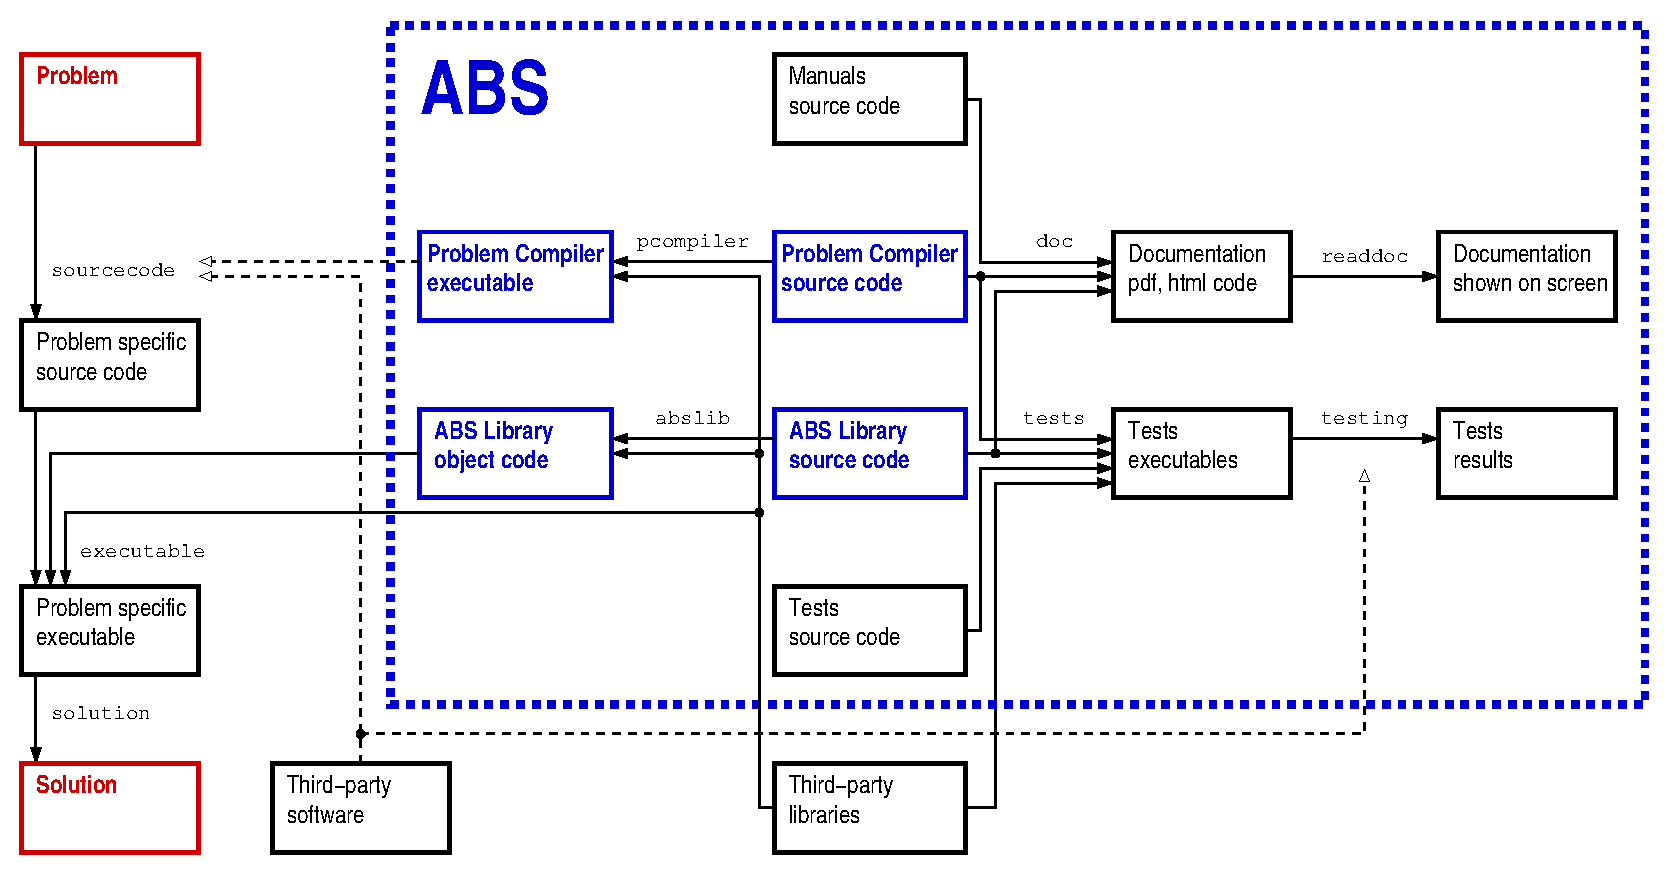
\includegraphics[width=.995\linewidth]{{{TeX_links/ImagesGlobal/ABS/ABSoverview}}}\\
$
\underbrace{\rule{.135\linewidth}{0pt}}_{%
\begin{minipage}{.135\linewidth}
\noindent\scriptsize\centering
example directory
\end{minipage}
}
$
\hspace*{\fill}
$
\underbrace{\rule{.06\linewidth}{0pt}}_{%
\text{\scriptsize global}
}
$
\hspace*{\fill}
$
\underbrace{\rule{.77\linewidth}{0pt}}_{%
\text{\scriptsize branch root}
}
$
\def\localcaptionFIRST{General structure, build process and operation of \ProjectAcronym}
\def\localcaptionSECOND{Solid arrows illustrate the build process;
dashed arrows show the influence of specific executables on the build
process}
\caption[\localcaptionFIRST.]%
{\label{fig:ABSoverview}%
\localcaptionFIRST\footnotemark.
\localcaptionSECOND.}
\makeatletter%
\global\let\localcaptionFIRST\@undefined%
\global\let\localcaptionSECOND\@undefined%
\makeatother%
\end{figure}\footnotetext{In addition to the dependencies illustrated,
building the ``Problem Specific executable'' requires access to ``ABS
Library source code'' to (re)build \texttt{main.o}. This is an artifact
of using the build tool \texttt{GPRbuild} \cite{gprbuildManual}.}


\ref{fig:ABSoverview} illustrates the general structure of \ProjectAcronym{}
and its application. The \concept{Problem Compiler} and the
\concept{ABS Library} are the core modules of \ProjectAcronym{}, which
implement functionality for the abstraction-based solution of
synthesis, analysis and verification problems for infinite state
dynamical systems. The remaining modules support the development and
maintenance of the software, and in particular, its
documentation and test. In addition to the aforementioned modules, the
branch root also contains some of the third-party libraries and
software on which \ProjectAcronym{} relies; see Section
\ref{s:SystemPrerequisites}.

Each problem that is to be solved using \ProjectAcronym{} requires its
own \concept{example directory} with a distinguished file containing
the problem description.
\ProjectAcronym{} will generate auxiliary and temporary files as well
as a file containing the solution in that directory.
(If there is no solution, failure is signaled.)

The build process of \ProjectAcronym{} as well as the process of
solving a problem using \ProjectAcronym{} is controlled using the tool
\verb|make| and the file \verb|Makefile| that resides at the root
level of the branch and of every example directory, respectively, in
which the most important targets are already illustrated in
\ref{fig:ABSoverview}.
% More details are given in Sections
% \ref{s:organization:Structure:TopLevelBuild} and
% \ref{s:organization:Structure:Application}.

\subsubsection{The Build Process of \ProjectAcronym}
\label{s:organization:Structure:TopLevelBuild}

At its root level, each branch contains the file \verb|Makefile|,
which controls the build process of \ProjectAcronym.
We describe the main targets, where the notion of a
\concept{debug variant} refers to executable and object files that
carry information useful for debugging, which is not present in the
\concept{release variants} of these files:
%\\[1ex]
%\noindent{\tabcolsep0pt%
\begin{center}
\renewcommand{\arraystretch}{1.3}%
\tabcolsep0pt%
\begin{tabularx}{.98\linewidth}{lp{10pt}X}
\texttt{make} or \texttt{make all} &&
Builds the whole of \ProjectAcronym{}:
Produces executable and object files for the third-party libraries and
software. Produces these files, each in a debug and a
release variant, for Problem Compiler, \ProjectAcronym{}
Library and tests.
Builds complete documentation for \ProjectAcronym.
\\
\texttt{make pcompiler} &&
Builds both the debug and the release variants of the Problem Compiler.
\\
\texttt{make abslib} &&
Builds both the debug and the release variants of the
\ProjectAcronym{} Library.
\\
\texttt{make tests} &&
Builds both the debug and the release variants of the tests.
\\
\texttt{make testing} &&
Runs both the debug and the release variants of all tests,
or of a subset of tests specified by an optional argument.
See Section \ref{s:Tests}.
\\
\texttt{make doc} &&
Builds complete documentation for \ProjectAcronym:
Generates \verb|pdf| files of the present
document and its companion document \cite{ABS_UsersManual}. Generates
the software reference documentation \cite{doxygenManual,gnatdocManual}
in the form of \verb|html| files from source code of the Problem
Compiler and the \ProjectAcronym{} Library.
\\
\texttt{make readdoc} &&
Opens the present document, its companion document
\cite{ABS_UsersManual}, and the software reference documentation using
the browser \texttt{firefox}.
\\
\texttt{make manuals} &&
Generates \verb|pdf| files of the present
document and its companion document \cite{ABS_UsersManual}.
\\
\texttt{make newproblem} &&
Generates and initializes a new example directory.
See Section \ref{s:organization:Structure:Application}.
\\
\texttt{make debug} &&
Builds the debug variants of Problem Compiler,
\ProjectAcronym{} Library and tests.
\\
\texttt{make release} &&
Builds the release variants of Problem Compiler,
\ProjectAcronym{} Library and tests.
\\
\texttt{make clean} &&
Produces executable and object files for the third-party libraries and
software.
Removes all executable and object files of Problem Compiler,
\ProjectAcronym{} Library and tests.
Removes auxiliary files created during the generation
of the present document and its companion document
\cite{ABS_UsersManual},
as well as software reference documentation files.
\\
\texttt{make cleanall} &&
Performs \texttt{make clean}, then removes executable and object files
for the third-party libraries and software.
\end{tabularx}%}\\
\end{center}

The commands described above can be used on any of the platforms
listed in \ref{tab:RemoteMachines} for which no restrictions are
given. \ProjectAcronym{} is then built for and run on your local
computer, using native compilation.
That is, the \concept{host platform}, which is associated
with the local computer being used for the build process, and the
\concept{target platform}, on which generated executables will run,
coincide. Executable and object files are produced only for that
platform, and similarly for the removal of those files. Executables
will be run on your local computer.
For remote native compilation, cross compilation and remote testing,
see Section \ref{s:organization:Structure:Platforms}.

The commands described above operate on files that are organized into
the following direct subdirectories of the branch root:
% \\[1em]
% \noindent{\tabcolsep0pt%
\begin{center}
\renewcommand{\arraystretch}{1.3}%
\tabcolsep0pt
\begin{tabularx}{.98\linewidth}{lp{10pt}X}
\verb|doc/| &&
All files related to the documentation of
\ProjectAcronym{}, which includes
\verb|tex| source code files of the present
document and its companion document \cite{ABS_UsersManual}, as well as
files produced using \verb|make doc|.
\\
\verb|bin/| and \verb|obj/| &&
All executable and object files, respectively, of the Problem
Compiler, of the \ProjectAcronym{} Library and of all tests.
\\
\verb|body/| and \verb|spec/| &&
Ada package body (C non-header source code) files and
Ada package specification (C header) files, respectively,
of the Problem Compiler, of the
\ProjectAcronym{} Library and of all tests.
\\
\verb|libs/| &&
Third party software as mentioned in Section
\ref{s:SystemPrerequisites}, including executable and object files
produced through a build process.
% After compiling the included packages,  
% the respective executable and library files 
% can be found in subdirectories of \verb|libs/|.
\\
\verb|examples/| &&
Distinguished problems suitable for the application of
\ProjectAcronym{}, each in its own example directory.
See Section \ref{s:organization:Structure:Application}.
\\
\verb|admin/| &&
Files specifying version names and the like. See Sections
\ref{s:CodingAndMaintenanceConventions:ResponsibilitiesOfProjectAdministrator:ReleasesAndVersionNaming}
and
\ref{s:CodingAndMaintenanceConventions:ResponsibilitiesOfProjectAdministrator:FilesAndDirectories}.
\\
\verb|templates/| &&
Template files used for, e.g. creating example directories.
\end{tabularx}%}\\
\end{center}

\noindent
The directories
\verb|bin/|,
\verb|obj/|,
\verb|body/| and
\verb|spec/|
contain subdirectories associated
with one of the platforms listed in Section
\ref{tab:RemoteMachines},
with one of the compiling modes that produce debug or release
variants, respectively,
with one of the two core modules (Problem Compiler or
\ProjectAcronym{} Library), and with subsystems \cite{gprbuildManual}
of the code, as detailed below:
\begin{center}
\renewcommand{\arraystretch}{1.1}%
\tabcolsep0pt
\begin{tabularx}{.995\linewidth}{lp{5pt}X}
\verb|bin/|$<$\textit{platform}$>$\verb|/|$<$\textit{cmode}$>$\verb|/| &&
No subdirectories.
Files not in repository.
\\
\verb|obj/|$<$\textit{subsys}$>$\verb|/|$<$\textit{module}$>$\verb|/|$<$\textit{platform}$>$\verb|/|$<$\textit{cmode}$>$\verb|/| &&
No subdirectories.
Files not normally in repository.
\\
$<$\verb|body|$|$\verb|spec|$>$\verb|/|$<$\textit{subsys}$>$\verb|/|$<$\textit{module}$>$\verb|/| &&
No restriction on structure.
Files in repository.
\end{tabularx}
\end{center}

\noindent
Here, \textit{platform} is one of the target triples listed in
\ref{tab:RemoteMachines},
\textit{cmode} is one of \verb|debug| or \verb|release|,
\textit{module} is one of \verb|ProblemCompiler| or \verb|ABSLibrary|,
and
\textit{subsys} takes one of the values given in the following table:
% \\[1em]
% \noindent{\tabcolsep0pt%
\begin{center}
\renewcommand{\arraystretch}{1.3}%
\tabcolsep0pt
\begin{tabularx}{\linewidth}{lp{5pt}|p{5pt}X}
\textit{subsys} &&& Comments
\\\hline
\verb|readwrite| &&&
Regular module functionality.
Ada package body and package specification files
(C non-header source code and header files, respectively) appear in pairs and
can normally be modified by any programmer.
Object files not in repository.
\\
\verb|readonly| &&&
Same as \verb|readwrite|, but
Ada package body and package specification files
(C non-header source code and header files, respectively) normally not writable; see Section
\ref{s:CodingAndMaintenanceConventions:ResponsibilitiesOfProjectAdministrator:FilesAndDirectories}.
Critical code; before modification a thorough discussion involving all
programmers is required.
\\
\verb|hidden| &&&
Same as \verb|readonly|, but Ada package body and C non-header source code files
normally missing (all missing, or none missing).
Proprietary or otherwise confidential code;
object files in repository.
\\
\verb|test_rw| &&&
Same as \verb|readwrite|, but test functionality.
Built and run using \verb|make tests| and \verb|make testing|,
respectively. See also Section \ref{s:Tests}.
\\
\verb|test_ro| &&&
Same as \verb|readonly|, but test functionality.
\end{tabularx}%}\\
\end{center}

\noindent
It is not possible to have several files with the same name in any
subdirectories of \verb|body/| and \verb|spec/|.
Moreover, compilation of different files must not lead to the same
object file.
See \cite[Section~2.2.2]{gprbuildManual}.

\subsubsection{Application to Solve Synthesis, Analysis and Verification problems}
\label{s:organization:Structure:Application}

Each synthesis, analysis or verification problem that is to be solved
using \ProjectAcronym{} requires its own \concept{example directory}.
Such directories are generated using 
\verb|make newproblem| in the branch root,
which produces command-line dialog boxes,
and initially contain the following files:
\begin{center}
\renewcommand{\arraystretch}{1.3}%
\tabcolsep0pt%
\begin{tabularx}{.98\linewidth}{lp{10pt}X}
$<$\textit{pname}$>$\verb|.abcs| &&
Problem description, where \textit{pname} coincides with the
name of the example directory.
Initially empty; problem should be specified using the
language described in \cite{ABS_UsersManual}.
\\
\verb|Makefile| &&
Controls the application of \ProjectAcronym{} to solve the problem, as
detailed below, using code from the branch from which the example
directory is created.
\\
\verb|problem_project.gpr| &&
Project file controlling the process of building
problem-specific executable and object files;
see Section \ref{s:organization:Structure:LowLevelBuild}.
\end{tabularx}
\end{center}

\noindent
Example directories are normally located outside any branch, with
the exception of some distinguished problems located in the
subdirectory \verb|examples/| of some branch root;
see Section \ref{s:organization:Structure:TopLevelBuild}.
Only in the latter case, the files listed above are in the repository.
We proceed to describe the main targets of the file \verb|Makefile|
in the example directory, which uses the file \verb|Makefile| in the
branch root from which the example directory has been gereated,
if necessary:
\begin{center}
\renewcommand{\arraystretch}{1.3}%
\tabcolsep0pt%
\begin{tabularx}{.98\linewidth}{lp{10pt}X}
\texttt{make} or \texttt{make all} &&
Solves the problem:
Produces problem-specific source code.
Builds problem-specific executable and object files, each in a debug
and a release variant. Runs the release variant of the
executable.
\\
\texttt{make sourcecode} &&
Produces problem-specific source code.
\\
\texttt{make executable} &&
Builds problem-specific executable and object files, each in a debug
and a release variant.
\\
\texttt{make solution} &&
Synonymous with \verb|make all|.
\\
\texttt{make clean} &&
Removes all problem-specific source code, executable, object and
results files, including the respective subdirectories.
\end{tabularx}
\end{center}

The commands described above produce executable and object files only
for the platform associated with the computer being used for
the build process, and similarly for the removal of those files.
Executables are run on the local computer either.
Remote native compilation, cross-compilation and remote execution of
problem-specific files is not possible\footnote{%
\textcolor{red}{Remote application to solve synthesis, analysis and
  verification problems would be useful. Requires some thinking.
}}.

The commands described above operate on files that are
organized into the following direct subdirectories of the example
directory, where \textit{platform} and \textit{cmode}
are as in Section \ref{s:organization:Structure:TopLevelBuild}:
\begin{center}
\renewcommand{\arraystretch}{1.3}%
\tabcolsep0pt
\begin{tabularx}{.98\linewidth}{lp{10pt}X}
$<$\verb|obj|$|$\verb|bin|$>$\verb|/|$<$\textit{platform}$>$\verb|/|$<$\textit{cmode}$>$\verb|/| &&
Problem-specific executable and object files.
No subdirectories, not in repository.
\\
\verb|SourceCodeFiles/| &&
Problem-specific source code files.
No restriction on structure, not in repository.
\\
\verb|Results/| &&
Files related to the solution of the problem.
No restriction on structure, not in repository.
\end{tabularx}
\end{center}

\subsubsection{Low-level Build Processes}
\label{s:organization:Structure:LowLevelBuild}

In Sections \ref{s:organization:Structure:TopLevelBuild} and
\ref{s:organization:Structure:Application} we have described the top
level of two build processes, which is controlled using the tool
\verb|make|.
At lower levels, build processes are controlled using \verb|make| and
\verb|GPRbuild| \cite{gprbuildManual}, both of which have their
strengths and weaknesses.
Specifically, \verb|GPRbuild| is preferable whenever Ada source code
is involved or part of the source code is missing or confidential;
see e.g.~\cite[Sections 2.3-2.4]{gprbuildManual}. On the other hand,
\verb|make| better facilitates the use of the tools
\verb|flex| \cite{FlexManual} and
\verb|bison| \cite{GNUBisonManual}.

\paragraph{\ProjectAcronym{} Library.}
Source code: Mainly Ada, some C.
Controlled using \verb|GPRbuild| and the following files,
where \textit{subsys} is as in Section
\ref{s:organization:Structure:TopLevelBuild}:
\begin{center}
\renewcommand{\arraystretch}{1.3}%
\tabcolsep0pt%
\begin{tabularx}{.98\linewidth}{lp{10pt}X}
\verb|spec/|$<$\textit{subsys}$>$\texttt{/\ProjectAcronym{}Library/}$<$\textit{subsys}$>$\verb|.gpr|
&&
Build process for subsystem \textit{subsys} of the
\ProjectAcronym{} Library.
\\
\verb|spec/|\texttt{\ProjectAcronym{}Library.gpr}
&&
Options common to all subsystems of the \ProjectAcronym{} Library.
Scenarios \cite[Sec.~2.4]{gprbuildManual} facilitate
compilation of source code files calling problem-specific functions,
which naive use of \verb|GPRbuild| would not permit.
\end{tabularx}
\end{center}
 
The subsystem \verb|hidden| is special in that Ada package body
and C non-header source code files are normally missing and instead the
repository contains object files; see Section
\ref{s:organization:Structure:TopLevelBuild}. The line
\begin{flushleft}
\verb|for Externally_Built use "true";|
\end{flushleft}
in the file \verb|hidden.gpr| ensures proper handling of this
situation. The file \verb|Makefile| in the branch root prompts the
removal of that line should Ada package body or C non-header source code files
be actually present in \texttt{body/hidden/\ProjectAcronym{}Library/},
in which case the object files are built as usual.

Typically, adding new code files to a subsystem does not require
modifying any \verb|gpr| files. (New packages using third party
libraries that are not yet included in the repository are an exception
in that they require modifying compiler and linker flags.)
However, the \verb|gpr| file of each subsystem contains one of the
lines listed below, which should be modified accordingly to avoid
warning messages.

\begin{center}
\renewcommand{\arraystretch}{1.1}%
\tabcolsep0pt%
\begin{tabularx}{.98\linewidth}{lp{10pt}X}
\verb|for Languages use ("ada");|
&&
Ada package body file present; no C non-header source code file.
\\
\verb|for Languages use ("C");|
&&
C non-header source code file present; no Ada package body file.
\\
\verb|for Languages use ("ada","C");|
&&
Ada package body and C non-header source code files present.
\end{tabularx}%}\\
\end{center}

\paragraph{Problem Compiler.}
Source code: C. Uses \texttt{bison} and \texttt{flex}.
Controlled using the tool \verb|make| and the file
\verb|spec/Makefile.ProblemCompiler|.
%Compiler flags for the debug and release 
%compiling mode are defined for this module of \ProjectAcronym{} in this file.
That file contains a list of source code files used; dependency
detection is properly implemented.

\paragraph{Application to Solve Synthesis, Analysis and Verification problems.}
Source code: Ada and C.
Controlled using the tool \verb|GPRbuild| and the file
\verb|problem_project.gpr|
in example directory.
Compiler flags specifying paths usually differ from the corresponding
flags in the \verb|gpr| files of the \ProjectAcronym{} Library.
The list following the line
\begin{flushleft}
\verb|for Source_Files use |
\end{flushleft}
contains those source code files produced in the subdirectory
\verb|SourceCodeFiles/| that are used by the \ProjectAcronym{} Library
in the branch from which the example directory has been generated. 

\subsubsection{Computing Platforms}
\label{s:organization:Structure:Platforms}

In Section \ref{s:organization:Structure:TopLevelBuild} we have
described a build process based on native compilation, where the
host and the target platforms coincide. To build \ProjectAcronym{} for
platforms different from the host platform, the commands described in
Section \ref{s:organization:Structure:TopLevelBuild} may be combined
with an additional argument of the form
\verb|TARGET=|$<$\textit{tplat}$>$.
Here, \textit{tplat} is the intended target platform, which is subject
to the restrictions in \ref{tab:RemoteMachines}.

If the target platform equals the host platform,
commands will be performed as described in Section
\ref{s:organization:Structure:TopLevelBuild}. Otherwise, executable
and object files will be produced for the target platform, and
similarly for the removal of those files.
The build process is based on \concept{remote native compilation} if
\ref{tab:RemoteMachines} does not list any restriction for the target
platform, and is otherwise based on \concept{cross compilation}.
Executables will be run on the associated example host given in
\ref{tab:RemoteMachines} (\concept{remote execution}).
For the commands \texttt{make doc}, \texttt{make readdoc} and
\texttt{make newproblem}, specifying a target platform has no effect.

% For example,
% \begin{flushleft}
% \verb|> make all TARGET=x86_64-suse-linux|
% \end{flushleft}
% creates executable and object files for the target platform
% \verb|x86_64-suse-linux|, regardless of the host platform. Testing
% will be performed either on your local computer or on \verb|uranus|.

To enable remote native compilation and remote execution,
follow the steps below and set up an \verb|ssh| communication protocol
\emph{by key exchange}, for each example host listed in
\ref{tab:RemoteMachines}. Of course, you need an account on each of
the hosts listed in \ref{tab:RemoteMachines}, and these hosts should
be reachable from your network environment.

\begin{enumerate}
\makeatletter
\def\labelenumi{\theenumi.)}
\def\theenumi{\arabic{enumi}}
\def\p@enumi#1{#1.)}
\makeatother
\item 
On your local computer run
\begin{flushleft}
\verb|> ssh-keygen -t rsa|
\end{flushleft}
If you are asked if
the file \verb|~/.ssh/id_rsa| or
the file \verb|~/.ssh/id_rsa.pub|
should be overwritten, make your decision or ask your system administrator.
If you proceed, answer all remaining queries by pressing the enter
key, and then run
\begin{flushleft}
\verb|> chmod 600 ~/.ssh/id_rsa|
\end{flushleft}
\item
\label{s:organization:Structure:Platforms:item:ForEachRemoteHost}
Log in to the remote host with IP
$<$\textit{host ip}$>$, using your account,
\begin{flushleft}
\verb|> ssh |$<$\textit{user name}$>$\verb|@|$<$\textit{host ip}$>$
\end{flushleft}
and enter your password, then run the following code, and finally exit
from the remote host:
\begin{flushleft}
\verb|> mkdir ~/.ssh| \\
\verb|> chmod 700 ~/.ssh| \\
\verb|> exit|
\end{flushleft}
\item
Back on your local computer, copy the public key to the remote host,
using your account:
\begin{flushleft}
\verb|> scp ~/.ssh/id_rsa.pub |$<$\textit{user name}$>$\verb|@|$<$\textit{host ip}$>$\verb|:./.ssh/| \\
\end{flushleft}
\item
On your local computer, choose a short name \textit{host name}
representing the remote host with IP \textit{host ip} on which your
user name is \textit{user name}, and run:
\begin{flushleft}
\verb|> echo "Host |$<$\textit{host name}$>$\verb|" >> ~/.ssh/config| \\
\verb|> echo "HostName |$<$\textit{host ip}$>$\verb|" >> ~/.ssh/config| \\
\verb|> echo "User |$<$\textit{user name}$>$\verb|" >> ~/.ssh/config| \\
\verb|> echo "IdentityFile ~/.ssh/id_rsa" >> ~/.ssh/config|
\end{flushleft}
\item
Log in to the remote host with IP
$<$\textit{host ip}$>$, using your account,
\begin{flushleft}
\verb|> ssh |$<$\textit{user name}$>$\verb|@|$<$\textit{host ip}$>$
\end{flushleft}
and enter your password, then run the following code, and finally exit
from the remote host:
\begin{flushleft}
\verb|> touch ~/.ssh/authorized_keys| \\
\verb|> cp ~/.ssh/authorized_keys ~/.ssh/authorized_keys.bak| \\
\verb|> cat ~/.ssh/id_rsa.pub >> ~/.ssh/authorized_keys| \\
\verb|> chmod 600 ~/.ssh/authorized_keys| \\
\verb|> rm ~/.ssh/id_rsa.pub| \\
\verb|> exit|
\end{flushleft}
\item
Back on your local computer, if everything went well you should be
able to log in to the remote host, by using the short name you have
chosen, and without being asked for a password:
\begin{flushleft}
\verb|> ssh |$<$\textit{host name}$>$
\end{flushleft}
To be able to connect to another remote host using the same keys,
restart from Step
\ref{s:organization:Structure:Platforms:item:ForEachRemoteHost}.
\end{enumerate}

% \begin{enumerate}[1.)]
% \item 
% Log in to the example host with IP
% $<$\textit{host ip}$>$, using your account,
% \begin{flushleft}
% \verb|> ssh |$<$\textit{user name}$>$\verb|@|$<$\textit{host ip}$>$
% \end{flushleft}
% and enter your password.
% \item 
% Run 
% \begin{flushleft}
% \verb|> ssh-keygen -t rsa|
% \end{flushleft}
% Answer all appearing queries by pressing the enter key.
% \item 
% Run
% \begin{flushleft}
% \verb|> cat .ssh/id_rsa.pub >> .ssh/authorized_keys| \\
% \verb|> chmod 600 .ssh/authorized_keys| \\
% \verb|> rm .ssh/id_rsa.pub| 
% \end{flushleft}
% \item
% Log-off using the command \verb|exit|.
% Back on your local computer run
% \begin{flushleft}
% \verb|> scp |$<$\textit{user name}$>$\verb|@|$<$\textit{host ip}$>$\verb|:.ssh/id_rsa .ssh/|$<$\textit{host name}$>$\verb|.rsa| 
% \end{flushleft}
% in your home directory and enter your password. Continue with
% \begin{flushleft}
% \verb|> chmod 600 .ssh/|$<$\textit{host name}$>$\verb|.rsa| \\
% \verb|> echo "Host |$<$\textit{host name}$>$\verb|" >> .ssh/config| \\
% \verb|> echo "HostName |$<$\textit{host ip}$>$\verb|" >> .ssh/config| \\
% \verb|> echo "User |$<$\textit{user name}$>$\verb|" >> .ssh/config| \\
% \verb|> echo "IdentityFile ~/.ssh/|$<$\textit{host name}$>$\verb|.rsa" >> .ssh/config|
% \end{flushleft}
% \end{enumerate}
% If everything went well you should be able to log in to the example
% host,
% \begin{flushleft}
% \verb|> ssh |$<$\textit{host name}$>$
% \end{flushleft}
% without being asked for a password.
% Otherwise, manually correct the file \verb|~/.ssh/config|.

\subsection{Program Structure}
\label{s:organization:ProgramStructure}

\subsubsection{Entry Point}

The entry point of a problem-specific executable file
is the Ada function \verb|Main| coded in \verb|body/public/main.adb|. 
The central data structures used in this file are the following:

\begin{center}
\renewcommand{\arraystretch}{1.2}%
\tabcolsep0pt
\begin{tabularx}{\linewidth}{lp{10pt}X}
Identifier in \texttt{main.adb} && Description
\\
\hline
\texttt{P} && Data structure for holding the user input and some auxiliary data, e.g. a priori enclosures. 
For more details see Section \ref{s:organization:ProgramFlowSemantics}.  \\
\texttt{G} && Data structure for holding the data related to growth bounds. \\
\texttt{Cover} && Data structure for representing the cover of the continuous state space. \\
\texttt{Input\_Values} && Data structure for representing the input set of the abstraction. \\
\texttt{Abstraction} && Data structure for representing the abstraction. \\
\texttt{Abstract\_Specification} && Data structure for representing the abstract specification. \\
\texttt{Solution} && Data structure for representing the solution of the problem. In particular, 
the abstract controller is represented provided that the problem has been solved.
\end{tabularx}
\end{center}

\ref{fig:programflow} shows the program flow in the executable file. The most relevant packages implementing the functionality 
in the boxes in \ref{fig:programflow} are listed in \ref{tab:Packages}. Of course, they may use other packages not listed in \ref{tab:Packages}. A complete list of the source code files can be found in the next subsection.
\begin{figure}
\centering
\usetikzlibrary{arrows}
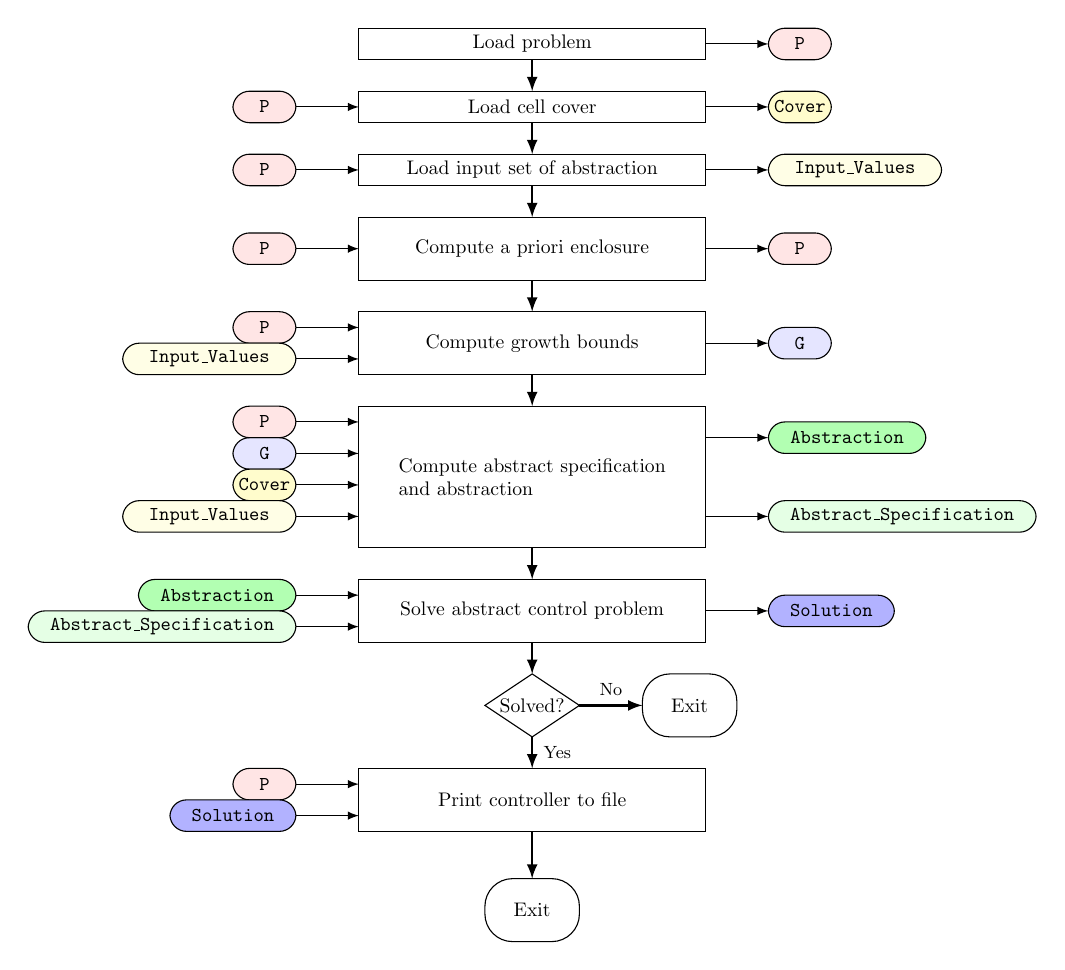
\begin{tikzpicture}[scale=0.8, every node/.style={scale=0.71}]
\coordinate (v1) at (0,-1.5) {} {};
\coordinate (v2) at (-0.75,-2) {} {};
\coordinate (v3) at (0,-2.5) {} {};
\coordinate (v4) at (0.75,-2) {} {};
\draw (v1) -- (v2) -- (v3) -- (v4) -- (v1);
\node (v5) at (0,-2) {Solved?};
\coordinate (v6) at (1.75,-2) {} {};
\draw [-latex,thick] (v4) -- (v6);
\draw [rounded corners=10pt] (1.75,-1.5) rectangle (3.25,-2.5) node[pos=0.5] {Exit};
\coordinate (v7) at (0,-3) {} {};
\draw [-latex,thick] (v3) -- (v7);
\draw [rounded corners=10pt] (-0.75,-4.75) rectangle (0.75,-5.75) node[pos=0.5] {Exit};
\draw [-latex] (-2.75,-3) rectangle (2.75,-4) node[pos=.5] {Print controller to file};
\coordinate (v8) at (0,-1) {} {};
\draw [-latex,thick] (v8) -- (v1);
\draw [-latex] (-2.75,0) rectangle (2.75,-1) node[pos=.5] {Solve abstract control problem};
\coordinate (v9) at (-3.75,-0.25) {} ;
\coordinate (v10) at (-2.75,-0.25) {};
\coordinate (v11) at (-3.75,-0.75) {} ;
\coordinate (v12) at (-2.75,-0.75) {} ;
\draw [rounded corners=6pt,fill=green!30] (-6.25,0) rectangle (-3.75,-0.5) node[pos=.5] {\texttt{Abstraction}};
\draw [rounded corners=6pt,fill=green!10] (-8,-0.5) rectangle (-3.75,-1) node[pos=.5] {\texttt{Abstract\_Specification}};
\draw [-latex] (v9) -- (v10);
\draw [-latex] (v11) -- (v12);
\draw [-latex] (-2.75,2.75) rectangle (2.75,0.5) node[pos=.5,align=left] {Compute abstract specification\\and abstraction};
\coordinate (v13) at (2.75,2.25) {} {};
\coordinate (v14) at (3.75,2.25) {} {};
\coordinate (v15) at (2.75,1) {};
\coordinate (v16) at (3.75,1) {};
\draw [rounded corners=6pt,fill=green!10] (-8+11.75,1.25) rectangle (-3.75+11.75,0.75) node[pos=.5] {\texttt{Abstract\_Specification}};
\draw [rounded corners=6pt,fill=green!30] (-6.25+10,2.5) rectangle (-3.75+10,2) node[pos=.5] {\texttt{Abstraction}};
\draw [rounded corners=6pt,fill=blue!10] (-4.75,2.25) rectangle (-3.75,1.75) node[pos=.5] {\texttt{G}};
\draw [-latex] (v13) -- (v14);
\draw [-latex] (v15) -- (v16);
\draw [rounded corners=6pt,fill=yellow!20] (-4.75,1.75) rectangle (-3.75,1.25) node[pos=.5] {\texttt{Cover}};
\draw [rounded corners=6pt,fill=yellow!10] (-6.5,1.25) rectangle (-3.75,0.75) node[pos=.5] {\texttt{Input\_Values}};
\draw [rounded corners=6pt,fill=red!10] (-4.75,2.75) rectangle (-3.75,2.25) node[pos=.5] {\texttt{P}};
\coordinate (v17) at (-3.75,2.5) {};
\coordinate (v18) at (-2.75,2.5) {};
\coordinate (v19) at (-3.75,2) {};
\coordinate (v20) at (-2.75,2) {};
\coordinate (v21) at (-3.75,1.5) {};
\coordinate (v22) at (-2.75,1.5) {};
\coordinate (v23) at (-3.75,1) {};
\coordinate (v24) at (-2.75,1) {};
\draw [-latex] (v17) -- (v18);
\draw [-latex] (v19) -- (v20);
\draw [-latex] (v21) -- (v22);
\draw [-latex] (v23) -- (v24);
\draw [-latex] (-2.75,6.75) rectangle (2.75,6.25) node[pos=.5] {Load input set of abstraction};
\draw [-latex] (-2.75,7.75) rectangle (2.75,7.25) node[pos=.5] {Load cell cover};
\coordinate (v25) at (-3.75,4) {} {} {};
\coordinate (v26) at (-2.75,4) {} {} {} {};
\draw [rounded corners=6pt,fill=red!10] (-4.75,4.25) rectangle (-3.75,3.75) node[pos=.5] {\texttt{P}};
\draw [-latex] (v25) -- (v26);
\coordinate (v27) at (2.75,6.5) {};
\coordinate (v28) at (3.75,6.5) {};
\draw [-latex] (v27) -- (v28);
\draw [rounded corners=6pt,fill=yellow!10] (3.75,6.75) rectangle (6.5,6.25) node[pos=.5] {\texttt{Input\_Values}};
\draw [rounded corners=6pt,fill=yellow!10] (-6.5,3.25) rectangle (-3.75,3.75) node[pos=.5] {\texttt{Input\_Values}};
\draw [-latex] (-2.75,4.25) rectangle (2.75,3.25) node[pos=.5] {Compute growth bounds};
\coordinate (v29) at (-3.75,3.5) {} {};
\coordinate (v30) at (-2.75,3.5) {} {};
\draw [-latex] (v29) -- (v30);
\coordinate (v31) at (2.75,3.75) {} {};
\coordinate (v32) at (3.75,3.75) {} {};
\draw [-latex] (v31) -- (v32);
\draw [rounded corners=6pt,fill=blue!10] (3.75,4) rectangle (4.75,3.5) node[pos=.5] {\texttt{G}};
\coordinate (v33) at (-3.75,6.5) {};
\coordinate (v34) at (-2.75,6.5) {};
\draw [-latex] (v33) -- (v34);
\draw [rounded corners=6pt,fill=red!10] (-4.75,6.75) rectangle (-3.75,6.25) node[pos=.5] {\texttt{P}};
\coordinate (v35) at (0,3.25) {} {};
\coordinate (v36) at (0,2.75) {};
\draw [-latex,thick](v35) -- (v36);
\coordinate (v37) at (0,0.5) {};
\coordinate (v38) at (0,0) {} {};
\draw [-latex,thick](v37) -- (v38);
\coordinate (v39) at (0,4.75) {};
\coordinate (v40) at (0,4.25) {};
\draw [-latex,thick] (v39) -- (v40);
\coordinate (v41) at (0,7.25) {} {} {};
\coordinate (v42) at (0,6.75) {} {} {};
\draw [-latex,thick] (v41) -- (v42);
\coordinate (v43) at (2.75,7.5) {};
\coordinate (v44) at (3.75,7.5) {};
\coordinate (v45) at (-3.75,7.5) {};
\coordinate (v46) at (-2.75,7.5) {};
\draw [-latex] (v43) -- (v44);
\draw [-latex] (v45) -- (v46);
\draw [rounded corners=6pt,fill=yellow!20] (3.75,7.75) rectangle (4.75,7.25) node[pos=0.5] {\texttt{Cover}};
\draw [rounded corners=6pt,fill=red!10] (-4.75,7.75) rectangle (-3.75,7.25) node[pos=0.5] {\texttt{P}};
\coordinate (v47) at (2.75,-0.5) {};
\coordinate (v48) at (3.75,-0.5) {};
\draw [-latex] (v47) -- (v48);
\draw  (-2.75,8.75) rectangle (2.75,8.25) node[pos=.5] {Load problem};
\coordinate (v49) at (2.75,8.5) {} {} {};
\coordinate (v50) at (3.75,8.5) {} {} {};
\draw[rounded corners=6pt,fill=red!10]  (3.75,8.75) rectangle (4.75,8.25) node[pos=.5] {\texttt{P}};
\draw[-latex]  (v49) -- (v50);
\coordinate (v51) at (0,8.25) {} {} {};
\coordinate (v52) at (0,7.75) {} {} {};
\draw[-latex,thick] (v51) -- (v52);
\node at (1.25,-1.75) {\small{No}};
\node at (0.4,-2.75) {\small{Yes}};
\coordinate (v53) at (0,-4) {};
\coordinate (v54) at (0,-4.75) {};
\draw[-latex,thick]  (v53) -- (v54);
\draw [rounded corners=6pt,fill=blue!30] (-8+11.75,1.25-1.5) rectangle (-6+11.75,0.75-1.5) node[pos=.5] {\texttt{Solution}};
\coordinate (v55) at (-3.75,-3.5-.25) {};
\coordinate (v56) at (-2.75,-3.5-.25) {};
\coordinate (w55) at (-3.75,-3.5+.25) {};
\coordinate (w56) at (-2.75,-3.5+.25) {};
\draw[-latex]  (v55) -- (v56);
\draw[-latex]  (w55) -- (w56);
\draw [rounded corners=6pt,fill=red!10] (-4.75,1.25-1.5-3+.25) rectangle (-3.75,0.75-1.5-3+.25) node[pos=0.5] {\texttt{P}};
\draw [rounded corners=6pt,fill=blue!30] (-8+2.25,1.25-1.5-3-.25) rectangle (-6+2.25,0.75-1.5-3-.25) node[pos=.5] {\texttt{Solution}};
\coordinate (v57) at (0,6.25) {} {};
\coordinate (v58) at (0,5.75) {} {};
\draw[-latex,thick]  (v57) -- (v58);
\draw  (-2.75,5.75) rectangle (2.75,4.75) node[pos=.5] {Compute a priori enclosure};
\coordinate (v59) at (-3.75,5.25) {};
\coordinate (v60) at (-2.75,5.25) {};
\coordinate (v61) at (2.75,5.25) {};
\coordinate (v62) at (3.75,5.25) {};
\draw[-latex]  (v59) -- (v60);
\draw[-latex]  (v61) -- (v62);
\draw[rounded corners=6pt,fill=red!10]  (-4.75,5.5) rectangle (-3.75,5) node[pos=0.5] {\texttt{P}};
\draw[rounded corners=6pt,fill=red!10]  (3.75,5.5) rectangle (4.75,5) node[pos=0.5] {\texttt{P}};
\end{tikzpicture}
\caption{\label{fig:programflow}The program flow of a problem-specific executable file.}
\end{figure}
%
\begin{table}
\tabcolsep0pt
\begin{tabularx}{\linewidth}{lp{10pt}X}
Label in \ref{fig:programflow} && Most relevant packages for the functionality \\
\hline
``Load problem" && \texttt{problem\_loading.adb} \\
``Load cell cover" && \texttt{cell\_cover.adb} \\
``Load input values" && \texttt{input\_values.adb} \\
``Compute a priori enclosure" && \texttt{apriori\_enclosure.adb} \\
 && \texttt{apriori\_enclosure\_aux.c} \\
``Compute growth bounds" && \texttt{growth\_bound.adb} \\
``Compute abstract specification and abstraction" && \texttt{abstraction\_i14sym.adb} \\
 && \texttt{abstraction\_i14sym-computation.adb} \\
 && \texttt{abstraction\_i14sym-predecessors.adb} \\
``Solve abstract control problem" && \texttt{dijkstra\_algorithm\_i13absoc.adb}\\
``Solved?" and ``Print controller to file" && \texttt{output\_results.adb} 
\end{tabularx}
\caption{\label{tab:Packages}Most relevant packages for the functionality depicted in \ref{fig:programflow}}
\end{table}

\subsubsection{Functionality of the Source Files}

We comment below on all packages of the branch. A more detailed description of the functionality of a package can be found in the software reference documentation. If a package consists of an
\verb|adb| and \verb|ads| file or a \verb|c| and a \verb|h| file then only the \verb|adb| and \verb|c| file, respectively,
is listed below.
\begin{center}
\renewcommand{\arraystretch}{1.2}%
\tabcolsep0pt%
\begin{tabularx}{.98\linewidth}{lp{10pt}X}
\texttt{abcs\_text\_io.adb} && Functions for printing messages on screen. \\
\texttt{abstraction\_i14sym.adb} && Functionality to read data associated to a computed abstraction, e.g. to read the predecessors of a given cell and input symbol. \\
\texttt{abstraction\_i14sym-computation.adb} \\
\texttt{abstraction\_i14sym-predecessors.adb} && Functionality to compute an abstraction according \cite{ReissigWeberRungger17}. \\
\texttt{apriori\_enclosure.adb}\\
\texttt{apriori\_enclosure\_aux.c} && Functionality to compute an a priori enclosure for the continuous-time dynamics. Interval arithmetic is used, which is only available in the C programming language.\\
\texttt{cell\_cover.adb} && Functionality to represent a cover of the continuous state space by hyper-intervals. \\
\texttt{controller\_i14sym.adb} && Functionality to read and write the data associated to a static controller.\\
\texttt{dijkstra\_algorithm\_i13absoc.adb} \\
\texttt{fifo.adb} && Functionality to solve the abstract control problem. \\
\texttt{established\_types.ads} && Basic type definitions. See Section \ref{s:organization:EstablishedTypes} for the details. \\
\texttt{grids.adb} && Functionality to represent a uniform grid on a real vector space. \\
\texttt{grids-data.adb} && Functionality to read and write data associated to elements of a uniform grid. \\
\texttt{grids-intersections.adb} && Functionality to perform intersection tests on a uniform grid with hyper-intervals.\\
\texttt{growth\_bound.adb} && Functionality to compute growth bounds according \cite{ReissigWeberRungger17}. \textcolor{blue}{Hao should add information here.} \\
\texttt{input\_values.adb} && Functionality to represent the abstract input set.\\
\texttt{main.adb} && Entry point of the program.\\
\texttt{output\_results.adb} && Functionality to print the results of the computation to files and screen.\\
\texttt{problem\_loading.adb} && Functionality to transfer the data from the problem-specific source code to the program. This file is closely related to \texttt{established\_types.adb} and the problem compiler.\\
\end{tabularx}
\end{center}

\subsubsection{Link between Problem Compiler and Program}
\label{s:organization:EstablishedTypes}

As already mentioned, the problem compiler generates source code to be used in the subsequent compilation process. 
Therefore, there exist function and variable declarations that are \emph{hard-coded} in the source code of 
the problem compiler but are defined in the package
\begin{verbatim}
established_types.ads
\end{verbatim}
Therefore, any change in this package requires at least checking 
the consequences for the output of the problem compiler.

\subsection{Semantics of the Program Flow}
\label{s:organization:ProgramFlowSemantics}

The crucial parts of the program with a focus on 
the interfaces between the different parts is 
depicted in \ref{fig:interfaces}. Below, we define semantics.

\subsubsection{Notation for Floating-point Arithmetic}
\label{s:NotationFloatingPointArithmetic}

Throughout this section, we will use the following notation and definitions.

\begin{center}
\renewcommand{\arraystretch}{1.1}%
\tabcolsep0pt%
\begin{tabularx}{.98\linewidth}{lp{10pt}X}
$\mathbb{F} \subseteq \mathbb{R}$ && Set of IEEE-754 double floating-point numbers \cite[Sec.~3.3.1]{MullerBrisebarreDeDinechinJeannerodLefevreMelquiondRevolStehle10} \\ 
$\operatorname{RN} \colon \mathbb{R} \to \mathbb{F} \cup \{-\infty,\infty\}$ && Round to nearest rounding operator \cite[Sec.~2.2.1]{MullerBrisebarreDeDinechinJeannerodLefevreMelquiondRevolStehle10} \\
$\oplus_{\operatorname{RN}}$ && Floating-point addition in the round to nearest mode \cite[Sec.~8.3]{MullerBrisebarreDeDinechinJeannerodLefevreMelquiondRevolStehle10} \\
$\ominus_{\operatorname{RN}}$ && Floating-point subtraction in the round to nearest mode \cite[Sec.~8.3]{MullerBrisebarreDeDinechinJeannerodLefevreMelquiondRevolStehle10} \\
$\otimes_{\operatorname{RN}}$ && Floating-point multiplication in the round to nearest mode \cite[Sec.~8.3]{MullerBrisebarreDeDinechinJeannerodLefevreMelquiondRevolStehle10} \\
$\oslash_{\operatorname{RN}}$ && Floating-point division in the round to nearest mode \cite[Sec.~8.3]{MullerBrisebarreDeDinechinJeannerodLefevreMelquiondRevolStehle10}
\end{tabularx}
\end{center}

\noindent
We assume operations on $\mathbb{F}$ to be evaluated from the left to
the right, e.g. $a \oplus b \oplus c = (a \oplus b) \oplus c$ for any $a, b, c \in \mathbb{F}$.

\begin{figure}
\centering
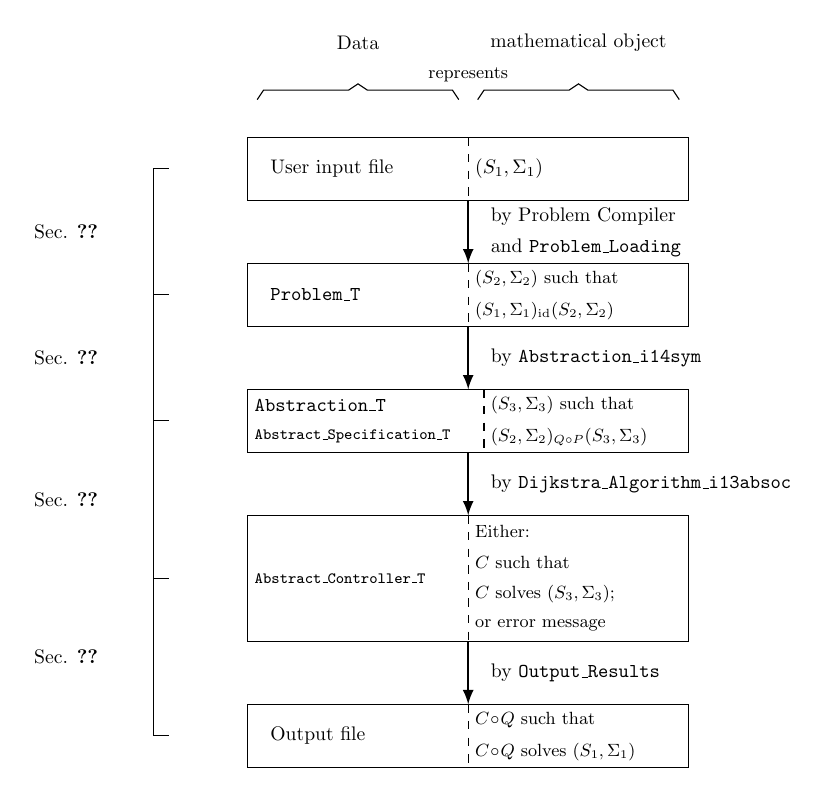
\begin{tikzpicture}[scale=0.8, every node/.style={scale=0.71}]
\newcommand{\offset}{3.5}
\draw  (-5,4.25) rectangle (2,3.25);
\node[right] at (-4.75,3.75) {\texttt{Problem\_T}};
\coordinate (v1) at (-1.5,4.25) {};
\coordinate (v2) at (-1.5,3.25) {};
\draw[dashed]  (v1) edge (v2);
\node[right] at (-1.5,4) {\small $(S_2,\Sigma_2)$ such that};
\draw  (-5,2.25) rectangle (2,1.25);
\coordinate (v3) at (-1.25,2.25) {} {};
\coordinate (w3) at (-1.5,2.25) {};
\draw [-latex,thick] (v2) -- (w3);
\node[right] at (-1.25,2.75) {by \texttt{Abstraction\_i14sym}};
\draw [-latex] (-5,6.25) rectangle (2,5.25);
\node[right] at (-1.25,4.5) {and \texttt{Problem\_Loading}};
%\draw [-latex] (1.5,7.25) rectangle (-4.75,8.25);
\node [right] at (-4.75,5.75) {User input file};
\node[right] at (-1.5,5.75) {$(S_1,\Sigma_1)$};
\coordinate (v6) at (-1.5,6.25) {};
\node[right] at (-1.25,5) {by Problem Compiler};
\coordinate (v7) at (-1.5,5.25) {};
\draw [-latex,thick] (v7) -- (v1);
\coordinate (w8) at (-1.5,1.25) {};
\coordinate (v8) at (-1.25,1.25) {} {};
\draw [dashed] (v3) -- (v8);
\node[right] at (-5,2) {\texttt{Abstraction\_T}};
\node[right] at (-1.25,2) {\small $(S_3,\Sigma_3)$ such that};
\draw [-latex] (-5,0.25) rectangle (2,-1.75);
\coordinate (v9) at (-1.5,0.25) {} {};
\coordinate (v10) at (-1.5,-1.75) {} {} {} {};
\draw [dashed] (v9) -- (v10);
\node[right] at (-5,-0.75) {\footnotesize\texttt{Abstract\_Controller\_T}};
\node[right] at (-1.5,0) {\small Either:};
\node[right] at (-1.5,-0.5) {\small $C$ such that};
\node[right] at (-1.5,-1) {\small $C$ solves $(S_3,\Sigma_3)$;};
\node[right] at (-1.5,-1.5) {\small or error message};
\draw [-latex,thick] (w8) -- (v9);
\draw [-latex] (-5,-2.75) rectangle (2,-3.75);
\node[right] at (-1.25,0.75) {by \texttt{Dijkstra\_Algorithm\_i13absoc}};
\node[right] at (-4.75,-3.25) {Output file};
\coordinate (v11) at (-1.5,-2.75);
\coordinate (v12) at (-1.5,-3.75);
\draw [dashed] (v11) -- (v12);
\node[right] at (-1.5,-3) {\small $C\!\circ\!Q$ such that};
\node[right] at (-1.5,-3.5) {\small $C\!\circ\!Q$ solves $(S_1,\Sigma_1)$};
\draw [dashed] (v6) -- (v7);
\node[right] at (-1.5,3.5) {\small $(S_1,\Sigma_1) \preccurlyeq_\mathrm{id} (S_2,\Sigma_2)$};
\node[right] at (-1.25,1.5) {\small $(S_2,\Sigma_2) \preccurlyeq_{Q \circ P} (S_3,\Sigma_3)$};
\draw [-latex,thick] (v10) -- (v11);
\node[right] at (-1.25,-2.25) {by \texttt{Output\_Results}};
\coordinate (v4) at (-5+.15,6.75+.1) {};
\coordinate (v5) at (-4.75,7) {};
\coordinate (v13) at (-3.5+.1,7) {};
\coordinate (v14) at (-3.25,7.25-.15) {};
\coordinate (v15) at (-3-.1,7) {};
\coordinate (v16) at (-1.75,7) {};
\coordinate (v17) at (-1.5-.15,6.75+.1) {};
\draw[] (v4) -- (v5) -- (v13) -- (v14) -- (v15) -- (v16) -- (v17);
\coordinate (a4) at (-5+.15+\offset,6.75+.1) {};
\coordinate (a5) at (-4.75+\offset,7) {};
\coordinate (a13) at (-3.5+.1+\offset,7) {};
\coordinate (a14) at (-3.25+\offset,7.25-.15) {};
\coordinate (a15) at (-3-.1+\offset,7) {};
\coordinate (a16) at (-1.75+\offset,7) {};
\coordinate (a17) at (-1.5-.15+\offset,6.75+.1) {};
\draw[] (a4) -- (a5) -- (a13) -- (a14) -- (a15) -- (a16) -- (a17);
\node at (-3.25,7.75) {Data};
\node at (-1.5,7.25) {\small represents};
\node at (0.25,7.75) {mathematical object};
\coordinate (v18) at (-6.25,5.75) {} {} {};
\coordinate (v19) at (-6.5,5.75) {} {} {};
\coordinate (v20) at (-6.5,3.75) {} {} {};
\coordinate (v21) at (-6.25,3.75) {} {} {};
\draw[] (v18) -- (v19) -- (v20) -- (v21);
\coordinate (v22) at (-6.5,1.75) {};
\coordinate (v23) at (-6.25,1.75) {};
\draw[] (v20) -- (v22) -- (v23);
\coordinate (v24) at (-6.5,-0.75) {};
\coordinate (v25) at (-6.25,-0.75) {};
\coordinate (v26) at (-6.5,-3.25) {};
\coordinate (v27) at (-6.25,-3.25) {};
\draw[] (v25) --(v24) -- (v26) -- (v27);
\draw[] (v24) -- (v22);
\node[right] at (-5,1.5) {\footnotesize\texttt{Abstract\_Specification\_T}};
\node[right] at (-8.5,4.75) {Sec. \ref{ss:user:problemt}};
\node[right] at (-8.5,2.75) {Sec. \ref{ss:problemt:abstraction}};
\node[right] at (-8.5,0.5) {Sec. \ref{ss:abstraction:controller}};
\node[right] at (-8.5,-2) {Sec. \ref{ss:controller:output}};
\makeatletter
\let\offset\@undefined
\makeatother
\end{tikzpicture}
\caption{\label{fig:interfaces}Interface definitions}
\end{figure}

\subsubsection{Interface definition: User input to \texttt{Problem\_T}}
\label{ss:user:problemt}

\subsubsection*{Formal requirement}

In what follows, we denote by $S_1$ the system $(\mathbb{R}^n,\mathbb{R}^n,U_1,U_1,\mathbb{R}^n,F_1,\operatorname{id})$ where $U_1 = U$, $F_1 = F$. Here and subsequently, $n$, $m$, $U$, $F$ are defined as in \cite[Section~2.1]{ABS_UsersManual}.
We denote by $\Sigma_1$ the reach-avoid specification associated with $(A_0,A_\mathrm{r},A_\mathrm{a})$ where the sets of the latter tuple are also defined as in \cite[Section~2.1]{ABS_UsersManual}.
We recall that the user specifies in the problem file the control problem $(S_1,\Sigma_1)$.
\\[1em]
The record \verb|P| of type \verb|Problem_T| in \verb|main.adb| shall represent a control problem $(S_2,\Sigma_2)$
such that
\begin{equation}
\label{e:frr:problemt}
(S_1,\Sigma_1) \preccurlyeq_{\operatorname{id}} (S_2,\Sigma_2).
\end{equation}
Here, $\operatorname{id}$ stands for the relation on $\mathbb{R}^n \times \mathbb{R}^n$ defined by $(x,y) \in \operatorname{id}$ iff $x=y$. $S_2$ is the system $(X_2,X_2,U_2,U_2,X_2,F_2,\operatorname{id})$, where
$X_2 = \mathbb{R}^n$, $U_2=U_1$ and 
$F_2 \colon X_2 \times U_2 \rightrightarrows X_2$ such that $F_2$ is a finite composition of elementary functions\footnote{See \cite[Section Grammar]{ABS_UsersManual} for the list of allowed elementary functions}. (So, the transition function of $S_1$ is transferred to a transition function being representable explicitly. 
Typically, the transition function of a sampled system is not representable explicitly.)
Moreover, $\Sigma_2$ is a reach-avoid specification associated with $(A_{2,0},A_{2,\mathrm{r}},A_{2,\mathrm{a}})$, where $A_{2,0},A_{2,\mathrm{r}},A_{2,\mathrm{a}} \subseteq \mathbb{F}^n$. (So, the specification $\Sigma_1$ is transferred to a specification defined on floating-point numbers.)


\subsubsection*{Established properties by the Problem Compiler}

The problem compiler in combination with the functionality in the package \verb|Problem_Loading| establishes \ref{e:frr:problemt} through the properties listed in \ref{tab:problemt}. 
%
We recall that the symbols $n,m,A_0,A_\mathrm{r},A_\mathrm{a}$ are defined as above, $z$, $w$, $\tau$ as in \cite[Section~2.1]{ABS_UsersManual}, 
$\segcc{x_\mathrm{min},x_\mathrm{max}}$ equals the operating range, and $\segcc{u_\mathrm{min},u_\mathrm{max}} = U_2 = U_1$. Here, $x_\mathrm{min},x_\mathrm{max} \in \mathbb{R}^n$, $x_\mathrm{min} < x_\mathrm{max}$ and $u_\mathrm{min},u_\mathrm{max} \in \mathbb{R}^m$, $u_\mathrm{min} \leq u_\mathrm{max}$. We recall that the user specifies an operating range.

In the column ``Symbol" of \ref{tab:problemt} we specify which symbol we use subsequently to denote the mathematical object represented by the corresponding entry of the record. 
\\[1em]
\begin{table}
\resizebox{\columnwidth}{!}{
\begin{tabular}{llll}
Identifier of entry of record \texttt{P} & Symbol & Set membership & Property \\
\hline 
\texttt{State\_Space\_Dimension} & & & equal to $n$ \\
\texttt{Input\_Space\_Dimension} & & & equal to $m$ \\
\texttt{xmin} & $x_{\mathrm{min},\circ}$ & $\mathbb{F}^n$ & $x_{\mathrm{min},\circ} \leq x_{\mathrm{min}}$ \\
\texttt{xmax} & $x_{\mathrm{max},\circ}$ & $\mathbb{F}^n$ & $x_{\mathrm{max},\circ} \geq x_{\mathrm{max}}$ \\
\texttt{umin} & $u_{\mathrm{min},\circ}$ & $\mathbb{F}^m$ & $u_{\mathrm{min},\circ} \geq u_{\mathrm{min}}$, $u_{\mathrm{min},\circ} \leq u_{\mathrm{max},\circ}$ \\
\texttt{umax} & $u_{\mathrm{max},\circ}$ & $\mathbb{F}^m$ & $u_{\mathrm{max},\circ} \leq u_{\mathrm{max}}$, $u_{\mathrm{min},\circ} \leq u_{\mathrm{max},\circ}$ \\
\texttt{List\_of\_periodic\_components} & $\ell$ & Power set of $\intcc{1;n}$ & See \ref{e:periodic:component} \\
\texttt{List\_of\_nonperiodic\_components} & $\bar \ell$ & Power set of $\intcc{1;n}$ & $\bar \ell = \intcc{1;n} \setminus \ell$ \\
\texttt{Initial\_State\_Space\_Subdivision} & $d_\mathrm{x}$ & $\mathbb{N}^n$ & \\
\texttt{Initial\_Input\_Space\_Subdivision} & $d_\mathrm{u}$ & $\mathbb{N}^m$ & \\
\texttt{Bounds\_of\_Dynamic\_Uncertainties} & $w_\circ$ & $\mathbb{F}_+^n$ & $w_\circ \geq w$ \\
\texttt{Bounds\_of\_Measurement\_Errors} & $z_\circ$ & $\mathbb{F}_+^n$ & $z_\circ \geq z$ \\
\texttt{Sampling\_Time} & $\tau_\circ$ & $\mathbb{F}_+$ & $\tau_\circ \defas \operatorname{RN}(\tau)$ \\
\texttt{Initial\_State\_Set} & $A_{2,0}$ & Power set of $\mathbb{F}^n$ & $A_{2,0} \supseteq A_0$ \\
\texttt{Target\_State\_Set} & $A_{2,\mathrm{r}}$ & Power set of $\mathbb{F}^n$ & $A_{2,\mathrm{r}} \subseteq A_{\mathrm{r}}$ \\
\texttt{Obstacle\_State\_Set} & $A_{2,\mathrm{a}}$ & Power set of $\mathbb{F}^n$ & $A_{2,\mathrm{a}} \supseteq A_{\mathrm{a}}$ \\
\texttt{General\_Solution\_Formula} & $\hat \varphi_\circ$ & & See \ref{e:error:in:phi},\ref{e:error:in:phicirc} \\
\texttt{Growth\_Bound\_Formula} & $\hat B_\circ$ & & See \ref{e:error:in:B},\ref{e:error:in:Bcirc}  \\
\texttt{Apriori\_Enclosure} & $K_1$ & Power set of $\mathbb{F}^n$ & See \ref{e:apriori:enclosure:state} \\
\texttt{Apriori\_Enclosure\_Growth\_Bounds} & $K_2$ & Power set of $\mathbb{F}^n$ & See \ref{e:apriori:enclosure:growth:bound} \\
\texttt{Rounded\_Initial\_State\_Radius} & $r_0$ & $\mathbb{F}_+^n$ & See \ref{e:initial:state:radius} \\
\texttt{Bounds\_of\_Lipschitz\_Matrices} & $\bar M$ & $\mathbb{F}^{n \times n}_+$ & See \ref{e:Lipschitz:Matrix:Bound} \\
\texttt{Bounds\_of\_Input\_Value\_Rounding\_Error} & $\eta_\mathrm{u}$ & $\mathbb{F}_+^m$ & See \ref{e:error:inputsignal} \\
\texttt{Bounds\_of\_Approximation\_Error\_of\_General\_Solution} & $\varepsilon_1$ & $\mathbb{F}_+^n$ & See \ref{e:error:in:phi} \\
\texttt{Bounds\_of\_Rounding\_Error\_of\_General\_Solution} & $\eta_1$ & $\mathbb{F}_+^n$ & See \ref{e:error:in:phicirc} \\
\texttt{Bounds\_of\_Approximation\_Error\_of\_Growth\_Bound} & $\varepsilon_2$ & $\mathbb{F}_+^n$ & See \ref{e:error:in:B} \\
\texttt{Bounds\_of\_Rounding\_Error\_of\_Growth\_Bound} & $\eta_2$ & $\mathbb{F}_+^n$ & See \ref{e:error:in:Bcirc} \\
\texttt{Bounds\_of\_Summation\_Error\_Growth\_Bound} & $\sigma_1$ & $\mathbb{F}_+^n$ & See \ref{e:error:addition:growth:bound} \\
\texttt{Bounds\_of\_Summation\_Error\_General\_Solution} & $\sigma_2$ & $\mathbb{F}_+^n$ & See \ref{e:error:addition} \\
\texttt{Bounds\_of\_Overapproximation\_Rounding\_Error} & $\sigma_3$ & $\mathbb{F}_+^n$ & See \ref{e:error:intersection:1}--\ref{e:error:intersection:4} \\
\texttt{Bounds\_of\_Overapproximation\_Radius} & $R$ & $\mathbb{F}^n_+$ &  See \ref{e:error:addition}
\end{tabular}%
}
\caption{\label{tab:problemt}Mathematical specification of the entries in the record.}
\end{table}
We now complete the information for \ref{tab:problemt}. 

\paragraph*{Initial state radius.}
$r_0 \in \mathbb{F}^n$ shall satisfy
\begin{equation}
\label{e:initial:state:radius}
\forall_{i \in \intcc{1;n}} : \ (r_0)_i \geq (x_\mathrm{max} - x_\mathrm{min})_i / (2d_\mathrm{x})_i.
\end{equation}

\paragraph*{Periodic components.}
Let $f$ be as in \cite[Section~2.1]{ABS_UsersManual},  
i.e. $f$ describes the unperturbed continuous-time dynamics.
Then, $\ell \subseteq \intcc{1;n}$ shall satisfy
\begin{equation}
\label{e:periodic:component}
\forall_{i \in \ell} \ \forall_{(x,u) \in \mathbb{R}^n \times U_1} \ f(x + p_i,u) = f (x,u),
\end{equation}
where $p_i \in \mathbb{R}^n_+$, $(p_i)_i = (x_{\mathrm{max}})_i-(x_{\mathrm{min}})_i$ and $(p_i)_j = 0$ for $j \neq i$.

We refer the reader to \cite[Sec.~VIII.D]{ReissigWeberRungger17} for the motivation for taking into account previous property of $f$.

\paragraph*{A priori enclosure for continuous-time dynamics.}
%Consider 
%\begin{equation}
%\label{e:unperturbed:rhs}
%\dot x = f(x,u),
%\end{equation}
%where $f$ is as above.
$K_1 \subseteq \mathbb{F}^n$ shall be convex such that for all $u \in U_1$, all $t \in \intcc{0,\tau}$ and any solution\footnote{See \cite[Sec.~VIII.A]{ReissigWeberRungger17} for the notion of solution in this context.} $\xi$ on $\intcc{0,t}$ of 
$\dot x \in f(x,u) + \segcc{-w_\circ,w_\circ}$ with input $u$ and $\xi(0) \in \segcc{x_\mathrm{min},x_\mathrm{max}}$ we have 
\begin{equation}
\label{e:apriori:enclosure:state}
\xi(\intcc{0,t}) \subseteq K_1.
\end{equation}

We refer the reader to \cite[Th.~VIII.5]{ReissigWeberRungger17} for the motivation for using an a priori enclosure.
\paragraph*{Bounds of Lipschitz matrices.}
$\bar M \in \mathbb{F}^{n \times n}_+$ shall satisfy
\begin{equation}
\label{e:Lipschitz:Matrix:Bound}
D_j f_i (K_1,U_1) \subseteq \intcc{-\bar M_{i,j},\bar M_{i,j}}
\end{equation}
for all $i,j \in \intcc{1;n}$, where $f$, $K_1$ and $U_1$ are as above.

We refer the reader to \cite[Th.~VIII.5]{ReissigWeberRungger17} for the motivation for using $\bar M$. 
An a priori enclosure is also required for estimating approximation errors \cite{Lohner88}.
\paragraph*{A priori enclosure for the growth bounds.}
Let us define 
\begin{align*}
B \colon \mathbb{R}_+ \times \mathbb{R}_+^n \times \mathbb{R}^{n \times n} \times \mathbb{R}_+^n &\to \mathbb{R}^n\\
(t,r,M,v) &\mapsto \e^{Mt}r + \int_{0}^t \e^{Ms}v \ ds.
\end{align*}
$K_2 \subseteq \mathbb{F}^n$ shall be such that
\begin{equation}
\label{e:apriori:enclosure:growth:bound}
B(\intcc{0,\tau},\segcc{0,r_0+z_\circ},M,\segcc{0,w_\circ}) \subseteq K_2
\end{equation}
for all $M \in \mathbb{R}^{n \times n}$ such that $-\bar M \leq M \leq \bar M$. The latter statement means $|M_{i,j}|\leq \bar M_{i,j}$ for all $i,j \in \intcc{1;n}$. 

We refer the reader to \cite[Th.~VIII.5]{ReissigWeberRungger17} for the motivation for using $B$.
\paragraph*{Floating-point implementation of the general solution.}
We first introduce 
the following functions, which are parametrized by 
$x,y \in \mathbb{R}^k$, $x\leq y$ and $x,y \in \mathbb{F}^k$, $x \leq y$, respectively, $k\in \mathbb{N}$. 
We comment on these functions after the definitions:
\begin{align*}
\operatorname{IndexedReals}_{x,y} \colon J_k & \to \mathbb{R}^k \\
(p,q) &\mapsto x + (p + (1, \ldots, 1)/2)\cdot (y - x)/q, 
\end{align*}
\begin{align*}
\operatorname{IndexedFloats}_{x,y} &\colon J_k  \to \mathbb{F}^k \\
(p,q) &\mapsto x \oplus_{\operatorname{RN}} (p \oplus_{\operatorname{RN}} (1, \ldots, 1)\oslash_{\operatorname{RN}}2)\otimes_{\operatorname{RN}} (y \ominus_{\operatorname{RN}} x)\oslash_{\operatorname{RN}}q,
\end{align*}
where
\begin{align*}
J_k \defas \{ (p,q) \in \mathbb{N}^k \times \mathbb{N}^k \mid \forall_{i \in \intcc{1;k}} \ p_i \in \intcc{0;q_i-1} \}.
\end{align*}
Roughly speaking, the only floating-point vectors with which we are allowed to work with are those obtained by $\operatorname{IndexedFloats}$. The reason is that the problem compiler is able to determine a bound on the rounding error between $\operatorname{IndexedReals}$ and $\operatorname{IndexedFloats}$ only. The use of those floating-point vectors is of significant importance for all formally correct computations. Images of the function $\operatorname{IndexedReals}$ are illustrated in \ref{fig:indexedreals}.
\begin{figure}
\centering
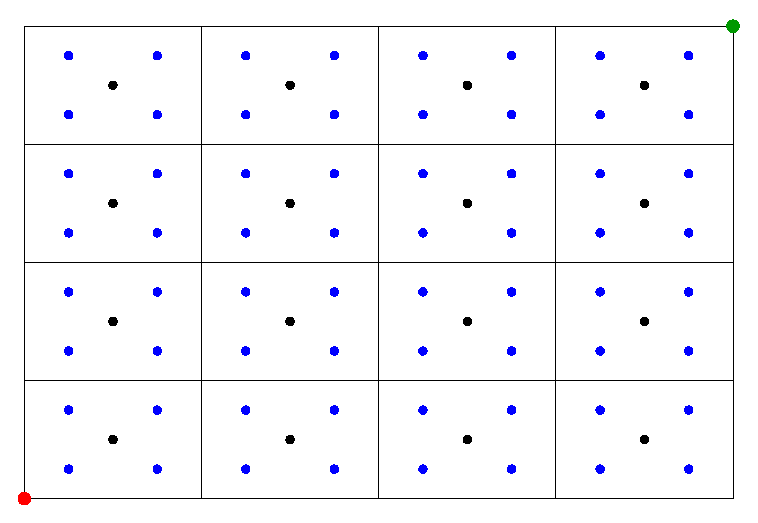
\includegraphics[scale=.5]{{{figures/IndexedReals}}}
\caption{\label{fig:indexedreals}Illustration of the function $\operatorname{IndexedReals}_{x,y}$ in $\mathbb{R}^2$, where $x$ and $y$ corresponds to the red and green colored point, respectively. The set of black and blue colored points corresponds to the image of $\operatorname{IndexedReals}_{x,y}(\cdot,(4,4))$ and $\operatorname{IndexedReals}_{x,y}(\cdot,(8,8))$, respectively. }
\end{figure}
\\
Consider 
\begin{equation}
\label{e:unperturbed:rhs}
\dot x = f(x,u),
\end{equation}
where $f$ is as above.
In the sequel, $\varphi$ denotes the general solution of \ref{e:unperturbed:rhs}. 
So, $\varphi(t,x,u)$ is the value of the general solution at time $t\in \mathbb{R}_+$ so that $\varphi(0,x,u) = x$ for all $(x,u) \in X_1 \times U_1$. 
%
A function $\hat \varphi \colon \dom \varphi \to \mathbb{R}^n$ and the constant $\varepsilon_1$ shall satisfy
\begin{align}
\label{e:error:in:phi}
\forall_{t \in \intcc{0,\tau} } & \nonumber \\
\forall_{(p,q) \in J_n \cap \tilde J_n } & \nonumber \\
\forall_{(p',q') \in J_m } & : \left | \hat \varphi(t,{\operatorname{Center}}(p,q),\operatorname{Signal}(p',q')) - \varphi(t,{\operatorname{Center}}(p,q),\operatorname{Signal}(p',q')) \right | \leq \varepsilon_1, 
\end{align}
\begin{figure}
\centering
\psfrag{a}[][]{$x_\mathrm{min}$}
\psfrag{b}[l][]{$x_\mathrm{max}$}
\psfrag{c}[l][]{$y$}
\includegraphics[scale=.5]{{{figures/IndexedRealsTree}}}
\caption{\label{fig:tree:auxiliary:endpoint} In case of a tree data structure, the root of the tree does \emph{not} correspond to $\segcc{x_\mathrm{min},x_\mathrm{max}}$ but to $\segcc{x_\mathrm{min},y}$. The reason is that aspect ratio of refined cells will coincide with the aspect ratio of the initial cells. }
\end{figure}
where here and subsequently
\begin{align*}
\tilde J_n & \defas \mathbb{N}^k \times ( \{ d_\mathrm{x} \} \cup \{ (2^{s+\nu},\ldots,2^{s+\nu}) \mid \nu \in \intcc{0;5} \} ), \\
\tilde u_\mathrm{min} & \defas u_\mathrm{min} - (\tilde u_\mathrm{max} - u_\mathrm{min} )/d_\mathrm{u}/2, \\
\tilde u_\mathrm{max} & \defas u_\mathrm{max} + (\tilde u_\mathrm{max} - u_\mathrm{min} )/d_\mathrm{u}/2, \\
y & \defas x_\mathrm{min} +  2^{s} \cdot (x_\mathrm{max}-x_\mathrm{min})/d_\mathrm{x}, \\
s &\defas \max_{i\in \intcc{1;n}} \min\{k \in \mathbb{Z}_+ \mid 2^k \geq (d_\mathrm{x})_i\},  \\
\operatorname{Signal}(p',q') &\defas \operatorname{IndexedReals}_{\tilde u_\mathrm{min},\tilde u_\mathrm{max}}(p',d_\mathrm{u} + (1,\ldots,1)),
\end{align*}
and
\begin{align}
\label{e:IndexedReals:Grid}
\operatorname{Center}(p,q) &\defas \operatorname{IndexedReals}_{x_\mathrm{min},x_\mathrm{max}}(p,d_\mathrm{x})
\end{align}
or
\begin{align}
\label{e:IndexedReals:Tree}
\operatorname{Center}(p,q) &\defas \operatorname{IndexedReals}_{x_\mathrm{min},y}(p,q).
\end{align}
Intuitively speaking, $\hat \varphi$ is an approximation formula to the general solution $\varphi$ 
and $\varepsilon_1$ bounds the respective approximation error. 
The particular choice of $y$ allow the use of a certain tree data structure for representing the abstract state space in the program. 
See \ref{fig:tree:auxiliary:endpoint}. 
The formula \ref{e:IndexedReals:Grid} is used for a grid-based cell covering 
while the formula \ref{e:IndexedReals:Tree} is used for a tree-based cell covering.

A floating-point implementation $\hat \varphi_\circ$ of $\hat \varphi$ shall satisfy:
\begin{align}
\label{e:error:in:phicirc}
\forall_{t \in \intcc{0,\tau} } &  \nonumber \\
\forall_{(p,q) \in J_n \cap \tilde J_n} & \nonumber \\
\forall_{(p',q') \in J_m } & : \left | {\hat \varphi_\circ} (\operatorname{RN}(t),{\operatorname{Center}}_\circ(p,q),{\operatorname{Signal}}_\circ(p',q')) - \hat \varphi(t,{\operatorname{Center}}(p,q),\operatorname{Signal}(p',q')) \right | \leq \eta_1, 
\end{align}
where here and subsequently
\begin{align*}
\tilde u_{\mathrm{min},\circ} & \defas u_{\mathrm{min},\circ} \ominus_{\operatorname{RN}} (u_{\mathrm{max},\circ} \ominus_{\operatorname{RN}} u_{\mathrm{min},\circ} ) \oslash_{\operatorname{RN}} d_\mathrm{u}  \oslash_{\operatorname{RN}} 2, \\
\tilde u_{\mathrm{max},\circ} & \defas u_{\mathrm{max},\circ} \oplus_{\operatorname{RN}} (u_{\mathrm{max},\circ} \ominus_{\operatorname{RN}} u_{\mathrm{min},\circ} ) \oslash_{\operatorname{RN}} d_\mathrm{u} \oslash_{\operatorname{RN}} 2, \\
y_\circ & \defas x_{\mathrm{min},\circ} \oplus_{\operatorname{RN}}  2^{s} \otimes_{\operatorname{RN}} (x_{\mathrm{max},\circ} \ominus_{\operatorname{RN}} x_{\mathrm{min},\circ}) \oslash_{\operatorname{RN}} d_\mathrm{x}, \\
\operatorname{Signal}_\circ(p',q') &\defas \operatorname{IndexedFloats}_{\tilde u_{\mathrm{min},\circ},\tilde u_{\mathrm{max},\circ}}(p',d_\mathrm{u} + (1,\ldots,1)),
\end{align*}
and
\begin{align}
\operatorname{Center}_\circ(p,q) &\defas \operatorname{IndexedFloats}_{x_{\mathrm{min},\circ},x_{\mathrm{max},\circ}}(p,d_\mathrm{x})
\end{align}
or
\begin{align}
\operatorname{Center}_\circ(p,q) &\defas \operatorname{IndexedFloats}_{x_{\mathrm{min},\circ},y_\circ}(p,q).
\end{align}
\paragraph*{Floating-point implementation of the growth bound formula.}
Similarly to $\varphi$, an approximation formula for $B$ is required: A function $\hat B$ and a constant $\varepsilon_2$ shall satisfy
\begin{align}
\label{e:error:in:B}
\forall_{t \in \intcc{0,\tau}} & \nonumber \\
\forall_{r \in \segcc{0, r_0+z_\circ}} &  \nonumber \\
\forall_{M \in \mathbb{F}^{n\times n} \text{ ess. non-negative s.t. } -\bar M \leq M \leq \bar M } & \nonumber\\
\forall_{v \in \segcc{0,w_\circ}} & :  \left | \hat B(t,r,M,v) - B(t,r,M,v) \right | \leq \varepsilon_2,
\end{align}
and $\hat B(t,r+z,M,v) = \hat B(t,z,M,v) + \hat B(t,r,M,0)$. The latter requirement is for allowing to store each summand separately. Note that $B$ possesses also the corresponding property. See also \ref{e:error:addition} below. \\
A floating-point implementation $\hat B_\circ$ of $\hat B$ shall satisfy
\begin{align}
\label{e:error:in:Bcirc}
\forall_{t \in \intcc{0,\tau}} &  \nonumber \\
\forall_{r \in \segcc{0, r_0+z_\circ} } & \nonumber \\
\forall_{M \in \mathbb{F}^{n\times n} \text{ ess. non-negative s.t. } -\bar M \leq M \leq \bar M } & \nonumber \\ 
\forall_{v \in \segcc{0,w_\circ} \cap \mathbb{F}^n } &: |\hat B_\circ ( \operatorname{RN}(t),\operatorname{RN}(r),M,v) - \hat B(t,r,M,v) | \leq \eta_2. 
\end{align}
\paragraph*{Floating-point implementation of the input signals.}
$\eta_\mathrm{u}$ satisfies
\begin{align}
\label{e:error:inputsignal}
\forall_{(p,q) \in J_m } : \  \operatorname{Signal}_\circ(p,q) \ominus_{\operatorname{RN}} \eta_\mathrm{u} \leq \operatorname{Signal}(p,q) \leq \operatorname{Signal}_\circ(p,q) \oplus_{\operatorname{RN}} \eta_\mathrm{u}. 
\end{align}
\paragraph*{Rounding error on addition in the growth bound formula.}
The constants $\sigma_1$ and $R_1$
\begin{align}
&\forall_{t \in \intcc{0,\tau} } &  \nonumber \\
&\forall_{r \in \segcc{0, r_0} } & \nonumber \\
&\forall_{M \in \mathbb{F}^{n\times n} \text{ ess. non-negative s.t. } -\bar M \leq M \leq \bar M }  \nonumber \\
& \forall_{\tilde z \in \segcc{0,z_\circ} \cap \mathbb{F}^n } \nonumber \\
& \forall_{v \in \segcc{0,w_\circ} \cap \mathbb{F}^n } \nonumber \\
&\forall_{\gamma_1 \in \segcc{0,\varepsilon_2} \cap \mathbb{F}^n} \nonumber \\
&\forall_{\gamma_2,\gamma_2' \in \segcc{0,\eta_2} \cap \mathbb{F}^n} : \nonumber \\
&\hat B_\circ(\operatorname{RN}(t),\operatorname{RN}(r),M,0)  + \gamma_2 + \hat B_\circ(\operatorname{RN}(t),\tilde z,M,v) + \gamma_2'  + \gamma_1  \nonumber  \\
& \leq  \hat B_\circ(\operatorname{RN}(t),\operatorname{RN}(r),M,0) \oplus_{\operatorname{RN}} \gamma_2 \oplus_{\operatorname{RN}} \hat B_\circ(\operatorname{RN}(t),\tilde z,M,v)\oplus_{\operatorname{RN}} \gamma_2' \oplus_{\operatorname{RN}}  \gamma_1 \oplus_{\operatorname{RN}} \sigma_1 \leq R_1.
\label{e:error:addition:growth:bound}
\end{align}
\paragraph*{Rounding error on addition associated with the general solution formula.}
The constants $\sigma_2$ and $R$ shall satisfy
\begin{align}
&\forall_{\gamma_1 \in \segcc{0,\varepsilon_1} \cap \mathbb{F}^n} \nonumber \\
&\forall_{\gamma_2 \in \segcc{0,\eta_1} \cap \mathbb{F}^n} \nonumber \\
&\forall_{\gamma_3 \in \segcc{0,R_1} \cap \mathbb{F}^n} \nonumber \\
&\gamma_1 + \gamma_2 + \gamma_3 \leq  \gamma_1 \oplus_{\operatorname{RN}} \gamma_2  \oplus_{\operatorname{RN}} \gamma_3 \oplus_{\operatorname{RN}} \sigma_2 \leq R.
\label{e:error:addition}
\end{align}
We would like to mention the following important property:
\begin{subequations}
\begin{align}
&\forall_{(p,q) \in J_n \cap \tilde J_n}\\
&\forall_{(p',q') \in J_m} \\
&\forall_{r \in \segcc{0, r_0} } \\
&\forall_{M \in \mathbb{F}^{n\times n} \text{ ess. non-negative s.t. } -\bar M \leq M \leq \bar M }
\end{align}
\label{e:assumptions}
\end{subequations}%
we have that
\begin{equation}
\label{e:overapproximation:Lipschitz}
\varphi(\tau,\operatorname{Center}(p,q),\operatorname{Signal}(p',q')) + \segcc{-B(\tau,r+z_\circ,M,w_\circ),B(\tau,r+z_\circ,M,w_\circ)}
\end{equation}
is a subset of
\begin{equation}
\label{e:overapproximation:Lipschitz:FP:without:sum}
\hat \varphi_\circ(\tau_\circ,\operatorname{Center}_\circ(p,q),\operatorname{Signal}_\circ(p',q')) + \segcc{-R,R}.
\end{equation}
Note that \ref{e:overapproximation:Lipschitz} is a general form of the overapproximation formula used in \cite[Th.~VIII.4]{ReissigWeberRungger17}. In contrast, \ref{e:overapproximation:Lipschitz:FP:without:sum} can be easily implemented on floating-point arithmetic in a formally correct manner. Of course, our statements also hold for the middle term in the inequalities \ref{e:error:addition} in place of $R$.

To prove our claim on the inclusion property for $R$, first use \ref{e:error:in:phi} and \ref{e:error:in:phicirc} to deduce that
\begin{equation}
|\varphi(\tau,\operatorname{Center}(p,q),\operatorname{Signal}(p',q')) - \hat \varphi_\circ(\tau_\circ,\operatorname{Center}_\circ(p,q),\operatorname{Signal}_\circ(p',q'))| \leq \varepsilon_1 + \eta_1
\end{equation}
under \ref{e:assumptions}.
Next, use \ref{e:error:in:B} to deduce 
\begin{equation*}
| B(\tau,r + z_\circ,M,w_\circ) - \hat B(\tau,r+z_\circ,M,w_\circ) | \leq \varepsilon_2 
\end{equation*}
and use \ref{e:error:in:Bcirc} to deduce
\begin{equation}
| \hat B(\tau,r+z_\circ,M,w_\circ) - (\hat B_\circ(\tau_\circ,r,M,0) + \hat B_\circ(\tau_\circ,z_\circ,M,w_\circ)) | \leq 2 \eta_2
\end{equation}
under \ref{e:assumptions}.
Finally, note that 
\begin{align*}
&\varphi(\tau,\operatorname{Center}(p,q),\operatorname{Signal}(p',q')) + B(\tau,r+z_\circ,M,w_\circ) \\ 
&\leq \hat \varphi_\circ(\tau_\circ,\operatorname{Center}_\circ(p,q),\operatorname{Signal}_\circ(p',q')) \\ & + \hat B_\circ(\tau_\circ,z_\circ,M,w_\circ) 
\\ & + \hat B_\circ(\tau_\circ,\operatorname{RN}(r),M,0) 
\\ & + \varepsilon_1 + \eta_1 + \varepsilon_2 + 2\eta_2 \leq \varphi_\circ(\tau_\circ,\operatorname{Center}_\circ(p,q),\operatorname{Signal}_\circ(p',q')) + R
\end{align*}
under \ref{e:assumptions}.
\paragraph*{Floating-point implementation of intersection tests.}
The form of the subsequent bounds is due to the particular form of the method to perform intersection tests. 
The underlying concept of the used intersection test method is depicted in \ref{fig:intersection}. 
Briefly, given a hyper-interval $H \defas x + \segcc{-r-z_\circ,r+z_\circ}$, $x \in \mathbb{R}^n$, $r \in \mathbb{R}^n_+$ we determine for each $i \in \intcc{1;n}$ the values
\begin{equation}
\label{e:intersection:lower}
\frac{x_i-r_i-(z_\circ)_i-(x_\mathrm{min})_i}{\eta_i}
\end{equation}
and 
\begin{equation}
\label{e:intersection:upper}
\frac{x_i+r_i+(z_\circ)_i-(x_\mathrm{min})_i}{\eta_i}
\end{equation}
respectively. From these values we determine all $k_i,l_i \in \mathbb{Z}$ so that
$x_i - r_i - (z_\circ)_i \in (x_\mathrm{min})_i + \intcc{k_i\eta_i,(k_i+1)\eta_i}$ and 
$x_i + r_i + (z_\circ)_i \in (x_\mathrm{min})_i + \intcc{l_i\eta_i,(l_i+1)\eta_i}$, respectively. From those integers we can easily deduce the cells intersecting (or being contained in) the hyper-interval $H$. $\sigma_3$ below shall account for the rounding errors committed in previous fractions.
\begin{figure}
\centering
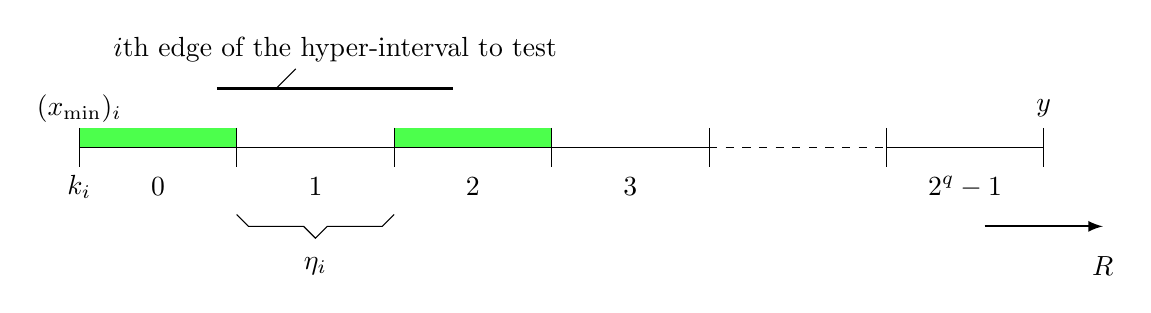
\begin{tikzpicture}
\coordinate (v5) at (-3.25,2.25) {} {} {};
\coordinate (v6) at (-1.25,2.25) {} {} {};
\coordinate (v4) at (-5.25,2.25) {} {} {};
\coordinate (v2) at (-7.25,2.25) {} {} {};
\coordinate (v7) at (0.75,2.25) {} {};
\coordinate (v1) at (-7.25,2.5) {} {} {};
\fill[fill=green!70]  (v1) rectangle (v4);
\coordinate (v3) at (-7.25,2) {} {} {};
\coordinate (v8) at (-5.25,2.5) {} {} {};
\coordinate (v9) at (-5.25,2) {} {} {};
\coordinate (v10) at (-3.25,2.5) {} {} {};
\coordinate (v11) at (-3.25,2) {} {} {};
\coordinate (v12) at (-1.25,2.5) {} {} {};
\fill[fill=green!70]  (v5) rectangle (v12);
\coordinate (v13) at (-1.25,2) {} {} {};
\coordinate (v14) at (0.75,2.5) {} {};
\coordinate (v15) at (0.75,2) {} {};
\draw[-] (v1) -- (v2) -- (v3);
\draw (v2) -- (v4) -- (v5) -- (v6) -- (v7);
\draw (v8) -- (v4) -- (v9);
\draw (v10) -- (v5) -- (v11);
\draw (v12) -- (v6) -- (v13);
\draw (v14) -- (v7) -- (v15);
\coordinate (v16) at (3,2.5) {} {};
\coordinate (v17) at (3,2.25) {} {};
\coordinate (v18) at (3,2) {} {};
\draw (v16) -- (v17) -- (v18);
\draw[dashed] (v7) -- (3,2.25);
\coordinate (v20) at (-4,3) {};
\coordinate (v19) at (-5.5,3) {};
\coordinate (v21) at (-2.5,3) {};
\draw[very thick] (v19) -- (v21);
\node at (-6.25,1.75) {$0$};
\node at (-4.25,1.75) {$1$};
\node at (-2.25,1.75) {$2$};
\node at (-0.25,1.75) {$3$};
\coordinate (v22) at (5,2.25) {};
\coordinate (v23) at (5,2.5) {};
\coordinate (v24) at (5,2) {};
\draw (v17) -- (v22);
\draw (v23) -- (v22) -- (v24);
\node at (4,1.75) {$2^q-1$};
\node at (-7.25,2.75) {$(x_\mathrm{min})_i$};
\coordinate (v25) at (-5.25,1.5-.1) {};
\coordinate (v26) at (-5-.1,1.25) {};
\coordinate (v27) at (-4.5+.1,1.25) {};
\coordinate (v28) at (-4.25,1+.1) {};
\coordinate (v31) at (-4-.1,1.25) {};
\coordinate (v29) at (-3.5+.1,1.25) {};
\coordinate (v30) at (-3.25,1.5-.1) {};
\draw (v25) -- (v26) -- (v27) -- (v28) -- (v31) -- (v29) -- (v30);
\node at (-4.25,0.75) {$\eta_i$};
\node at (-4,3.5) {$i$th edge of the hyper-interval to test};
\coordinate (v32) at (-4.75,3) {} {};
\coordinate (v33) at (-4.5,3.25) {} {};
\draw[thin] (v32) -- (v33);
\coordinate (v34) at (4.25,1.25) {};
\coordinate (v35) at (5.75,1.25) {};
\node at (5.75,0.75) {$\mathbb{R}$};
\draw[thick,-latex]  (v34) -- (v35);
\node at (-7.25,1.75) {$k_i$};
\node at (5,2.75) {$y$};
\end{tikzpicture}
\caption{\label{fig:intersection}Illustration of the method for the intersection test. The green intervals are determined through the terms in \ref{e:intersection:lower} and \ref{e:intersection:upper}.}
\end{figure}
In particular, $\sigma_3$ shall satisfy:
\begin{align}
\label{e:error:intersection:1}
&\forall_{x \in \mathbb{F}^n \text{ s.t. } \exists_{(p,q) \in J_n \cap \tilde J_n} \exists_{(p',q') \in J_m} \  x = \hat \varphi_\circ(\tau_\circ,\operatorname{Center}_\circ(p,q),\operatorname{Signal}_\circ(p',q')) } \nonumber \\
&\forall_{r \in \segcc{0,R} \cap \mathbb{F}^n } \nonumber \\
&((x \ominus_{\operatorname{RN}} (r \oplus_{\operatorname{RN}} z_\circ) \ominus_{\operatorname{RN}} x_{\mathrm{min},\circ}  ) \oslash_{\operatorname{RN}} \eta_\circ) \ominus_{\operatorname{RN}} \sigma_3 \leq ((x-r-z_\circ-x_{\mathrm{min}})/\eta),
\end{align}
\begin{align}
\label{e:error:intersection:2}
&\forall_{x \in \mathbb{F}^n \text{ s.t. } \exists_{(p,q) \in J_n \cap \tilde J_n} \exists_{(p',q') \in J_m} \  x = \hat \varphi_\circ(\tau_\circ,\operatorname{Center}_\circ(p,q),\operatorname{Signal}_\circ(p',q')) } \nonumber \\
&\forall_{r \in \segcc{0,R} \cap \mathbb{F}^n  } \nonumber \\
&((x \oplus_{\operatorname{RN}} (r \oplus_{\operatorname{RN}} z_\circ) \ominus_{\operatorname{RN}} x_{\mathrm{min},\circ}  ) \oslash_{\operatorname{RN}} \eta_\circ) \oplus_{\operatorname{RN}} \sigma_3 \geq ((x+r+z_\circ-x_{\mathrm{min}})/\eta),
\end{align}
\begin{align}
\label{e:error:intersection:3}
\forall_{x \in (A_{2,0} \cup A_{2,\mathrm{r}} \cup A_{2,\mathrm{a}}) \cap \mathbb{F}^n}: \ 
((x \ominus_{\operatorname{RN}} x_{\mathrm{min},\circ}  ) \oslash_{\operatorname{RN}} \eta_\circ) \ominus_{\operatorname{RN}} \sigma_3 \leq ((x-x_{\mathrm{min}})/\eta),
\end{align}
\begin{align}
\label{e:error:intersection:4}
\forall_{x \in (A_{2,0} \cup A_{2,\mathrm{r}} \cup A_{2,\mathrm{a}}) \cap \mathbb{F}^n}: \ 
((x \ominus_{\operatorname{RN}} x_{\mathrm{min},\circ}  ) \oslash_{\operatorname{RN}} \eta_\circ) \oplus_{\operatorname{RN}} \sigma_3 \geq ((x-x_{\mathrm{min}})/\eta),
\end{align}
where $\eta = (x_\mathrm{max} - x_\mathrm{min}) / d_\mathrm{x}$, $\eta_\circ = ( x_{\mathrm{max},\circ} \ominus_{\operatorname{RN}} x_{ \mathrm{min},\circ} ) \oslash d_\mathrm{x}$ or $\eta = (y - x_\mathrm{min}) / q$, $\eta_\circ = ( y_\circ \ominus_{\operatorname{RN}} x_{ \mathrm{min},\circ} ) \oslash q$, $q \in \{ (2^{s+\nu},\ldots,2^{s+\nu}) \mid \nu \in \intcc{0;5} \}$. (Here, the divisions are understood component-wise and $y$, $y_\circ$ are as in previous paragraphs.)
\subsubsection{Interface definition: \texttt{Problem\_T} to \texttt{Abstraction\_T} and\\ \texttt{Abstract\_Specification\_T}}
\label{ss:problemt:abstraction}
The record of type \texttt{Abstraction\_T} shall represent a system $S_3 = (X_3,X_3,U_3,U_3,X_3,F_3,\operatorname{id})$ such that $X_3$ is finite,
\begin{equation*}
\exists_{\bar X_3 \subseteq X_3} : \ \bigcup_{x_3 \in \bar X_3} x_3 = \segcc{x_\mathrm{min},x_{\mathrm{max}}}
\end{equation*}
and
\begin{equation*}
S_2 \preccurlyeq_{Q\circ P} S_3,
\end{equation*}
where $P \colon \mathbb{R}^n \rightrightarrows \mathbb{R}^n$, $x \mapsto x + \segcc{-z_\circ, z_\circ}$ and $(x,y) \in Q$ iff $x \in y$.
The record of type \texttt{Abstract\_Specification\_T} shall represent a specification
$\Sigma_3$ on $S_3$ that is associated to a reach-avoid control problem $(A_{3,0},A_{3,\mathrm{r}},A_{3,\mathrm{a}})$ such that $(S_2,\Sigma_2) \preccurlyeq_{Q\circ P} (S_3,\Sigma_3)$.

\subsubsection{Interface definition: \texttt{Abstraction\_T} and \texttt{Abstract\_Specification\_T}\\ to \texttt{Abstract\_Controller\_T}}
\label{ss:abstraction:controller}

The record of type \texttt{Abstract\_Controller\_T} shall represent either a system $C$ such that $C$ solves $(S_3,\Sigma_3)$ or $C = \emptyset$.

\subsubsection{Interface definition: \texttt{Abstract\_Controller\_T} to Output file}
\label{ss:controller:output}

\noindent
\textcolor{red}{To be written.}

\section{Coding and Maintenance Conventions}
\label{s:CodingAndMaintenanceConventions}

\subsection{Using the Repository}
\label{s:CodingAndMaintenanceConventions:Repository}

\begin{enumerate}
\item
Update and commit operations should always be performed at the branch
level or some higher level to avoid inconsistencies.
\item
Branches are created, and handled, using ``cheap'' versions of the
respective operations whenever possible \cite{svnManual11}.
\item
Use locks sparingly. Avoid breaking or stealing locks whenever
possible \cite{svnManual11}.
\newcounter{myitemcounter}\setcounter{myitemcounter}{\value{enumi}}
\end{enumerate}

\noindent
The following additional rules apply to the trunk:

\begin{enumerate}
\setcounter{enumi}{\value{myitemcounter}}
%\makeatletter\global\let\c@myitemcounter\@undefined\makeatother
\item
Any branch should be consistent at any time:
\begin{itemize}
\item
In the branch root, the command \verb|make all| runs successfully
without any warnings or errors, except for warnings
generated by processing \TeX{} files,
on all platforms listed in Section \ref{s:SystemPrerequisites}.
\item
The command \verb|make testing| runs successfully without any warnings
or errors,
on all platforms listed in Section \ref{s:SystemPrerequisites}.
\item
The functioning of the source code is described correctly and in
sufficient detail by the comments in the source code, the manuals
\cite{ABS_UsersManual}, \cite{ABS_ProgrammersManual} and the reference
documentation (see Section
\ref{s:temporary:GenerationOfSoftwareReferenceDocumentation}).
\end{itemize}
\end{enumerate}

\subsection{Source Code Coding Policy}
\label{s:CodingAndMaintenanceConventions:SourceCode}

\begin{enumerate}
% \makeatletter
% \def\labelenumi{\theenumi.)}
% \def\theenumi{\arabic{enumi}}
% \def\p@enumi#1{#1.)}
% \makeatother
\item
\textcolor{red}{Hao, the meaning of the following rule is still not
  clear to me (nested ``except''; to which case does ``latter'' refer;
  does the first character of a word have to be a letter, or what is a
  word? etc.). Please
  clarify. In addition, did we really agree that identifiers for
  constants should be uppercase?}
\textcolor{blue}{Answer(Hao): Writing in uppercase for constants is a style
  that inherited from C. I reviewed the Ada book again and found that just first
  character of a letter is in uppercase even for constants. So let us agree on
  that constants takes the same style of the basic rule. By the way, I still
  advise using the same rule for variables so that we have a uniform style.}

  The basic rule for writing identifiers is beginning with a or more letters
  or a word then
  possibly followed by one or more letters, one or more words, one or more
  digits with embedded isolated underscores, in which the first character of
  a letter or word and only the first is in uppercase. For instance, the
  following are legal: 
  \verb|E, Err, Error, Free_State_Space, Free_S_1, Free_Space_12|. 
  \par
  (This rule applies for all identifiers except for \verb|variables|. For
  \verb|variables|,  we leave programmers themselves to decide. Please explain
  your identifiers in comment if they are not words).   
\item
  Identifiers for types defined by programmers include a suffix ``\verb|_T|''.
\item
  In the parameter list of a \texttt{procedure} in \texttt{Ada} or a
  \texttt{function} in \texttt{C}, the output parameter (if it has in
  \texttt{function} of \texttt{C}) occupies the first position.  
\end{enumerate}

\subsection{Source Code Documentation Policy}
\label{s:CodingAndMaintenanceConventions:SouceCodeDocumentation}

\begin{enumerate}%[(i)]
\item
Comment on every entry of a \verb|struct| or \verb|union| in C and a \verb|record| in Ada
\item 
Comment on every argument of a function/method/procedure unless the role of the argument is obvious 
\item 
Explain the functionality of every function/method/procedure in such a way that a third person understands
the use without having to read the implementation
\item 
Comment on the assumptions made to execute a function/method/procedure as intended
\item 
Comment on exceptions that may be raised explicitly
\end{enumerate}
\begin{Note}
One may experience some counter-intuitive behavior of the Ada documentation tool. 
Therefore, one should always check the produced output.
\end{Note}

\textcolor{red}{does this refer to the software ref doc only? or only
  to using comments in source codes?}\\
\textcolor{red}{svn in comments}

\subsection{Software Reference Documentation}
\label{s:temporary:GenerationOfSoftwareReferenceDocumentation}
\textcolor{red}{GR: I am not sure this information belongs into
  Section \ref{s:CodingAndMaintenanceConventions}.}

Software reference documentation is produced using the tool \verb|doxygen| for C source code and \verb|gnatdoc| for Ada source code.
To generate the software reference documentation run
\begin{verbatim}
make doc
\end{verbatim}
in the branch root. The automatically generated \verb|html| files are included in the directory \verb|doc/ProblemCompiler/html/| and \verb|doc/ABSLibrary/|. 
%
%
The files 
\begin{itemize}%[]
\item \verb|doc/ABSLibrary/index.html|, and
\item \verb|doc/ProblemCompiler/html/index.html|
\end{itemize}
are the entry points of the documentations. 
When \verb|firefox| is available on your system then run
\begin{verbatim}
make readdoc
\end{verbatim}
to open these files directly with \verb|firefox|. 

\subsection{Manuals}

\noindent
must be readable even if processed using \verb|dvips -t letter|, and
if printed on letter paper
\\
should be American English
\\
userman: must compile externally (arxiv)
\\
references (to equations, items etc): MUST be symbolic using \verb|\ref| and
the like
\\
\textcolor{red}{svn in comments: analogous with Section }


\subsection{Responsibilities of the Project Administrator}
\label{s:CodingAndMaintenanceConventions:ResponsibilitiesOfProjectAdministrator}

\subsubsection{Releases and Version Naming}
\label{s:CodingAndMaintenanceConventions:ResponsibilitiesOfProjectAdministrator:ReleasesAndVersionNaming}

For each branch, the file
\verb|admin/version_info_private.txt| contains a
\concept{version name} and an extended regular expression
\cite[Ch.~9]{IEEE1003.1_2008} to be satisfied by the version name;
the current values are \expandafter\verb\expandafter|\VersionName| and
\expandafter\verb\expandafter|\VersionNameRegularExpression|.
The file is maintained by the project administrator.

Version names are inherited by copied branches, and so different
branches may share a common version name. If the regular expression is
modified, the resulting expression should represent a stricter
condition than the expression from which it was derived. Version names
should be modified in such a way that the modification is intuitively
received as an increment. The version's \concept{main name} and
\concept{subname} is the part of the version name preceding and
following, respectively, the dot.

A \concept{release} is a deployable branch which is deemed to
represent an important stage of the development. If it is provided for
use outside of the development team, a release is called
\concept{public}; otherwise it is called \concept{internal}.
The conventions specified in Section
\ref{s:CodingAndMaintenanceConventions:Repository} for the trunk shall
analogously apply to any release.
The procedure by which the administrator declares a branch as a
release should follow the general approach in Section ``Release
Branches`` in \cite[Ch.~4]{svnManual11}, with the following additions:

\begin{enumerate}
\item
An internal release is generated by copying the trunk to the
subdirectory
\verb|branches/|,
where the copy will go under the name
\verb|release_|$<$version's main name of main development branch$>$.
To this end, if the version name of main development branch is
\VersionName{}, the following command should be run in the
working copy of the project root:
\begin{flushleft}
\verb|> svn cp ^/ABS/trunk ^/ABS/branches/release_|\expandafter\verb\expandafter|\VersionMainName |
\verb|-m "ABS version |\expandafter\verb\expandafter|\VersionMainName |\verb|released"|
\end{flushleft}
Afterwards, the version's main name of the main development branch is
incremented. Bugs in internal releases may be fixed using the existing
branch of the release.
\item
A public release is generated by copying an internal release to
\verb|tags/public/|,
where the copy will go under the name
\verb|release_|$<$version name of internal release$>$.
To this end, the following command should be run in the
working copy of the project root:
\begin{flushleft}
\verb|> svn cp ^/ABS/branches/release_|\expandafter\verb\expandafter|\VersionMainName |
\verb|^/ABS/tags/public/release_|\expandafter\verb\expandafter|\VersionName |
\verb|\|\\
\verb|> -m "ABS release |\expandafter\verb\expandafter|\VersionName |\verb|made public"|\\
\verb|> svn up|
\end{flushleft}
Afterwards, the version's subname of the original, internal release is
incremented.
\item
A public release is actually made available to the public as follows:
\\
First, the branch root of the public release is copied to the
location given in \cite[Section ``Quick Start'']{ABS_UsersManual}.
To this end, the following command should be run in the
working copy of the project root:
\begin{flushleft}
\verb|> svn rm ^/ABS/tags/public/CurrentPublicVersion/trunk |\verb|\|
\verb|> -m "^/ABS/tags/public/CurrentPublicVersion/trunk removed"|\\
\verb|> svn cp ^/ABS/tags/public/release_|\expandafter\verb\expandafter|\VersionName |
\verb|^/ABS/tags/public/CurrentPublicVersion/trunk |
\verb|\|\\
\verb|> -m "^/ABS/tags/public/CurrentPublicVersion/trunk linked to public release |
\expandafter\verb\expandafter|\VersionName"|\\
\verb|> svn up|
\end{flushleft}

Second, a user's manual should be provided, sharing
the version's main name given on its title page.
To this end, \verb|make manuals| is run in the working copy of the
publicly available branch
\verb|^/ABS/tags/public/CurrentPublicVersion/trunk|.
Afterwards, in the root directory of the working
copy of the administrator's web page, the following is run:
\begin{flushleft}
\verb|>| \verb|/bin/ln -f |
$<$\textit{full path of working copy of project root}$>$\verb| \|\\
\verb|>| \verb|/tags/public/CurrentPublicVersion/trunk/doc/Manuals/texfiles/usermanual.pdf \|\\
\verb|> ./pubs/ABSusersmanual.pdf|
\end{flushleft}
Now, the the working copy of the administrator's web page is
published.
\item
Finally, the following command should be run in the working copy of
the project root, to finish the creation of releases:
\begin{flushleft}
\verb|> svn commit trunk branches/release_|\expandafter\verb\expandafter|\VersionMainName tags/public/ \|\\
\verb|> -m "ABS: finished publication of release |\expandafter\verb\expandafter|\VersionName|\verb|"|
\end{flushleft}
\end{enumerate}

\subsubsection{Files and Directories}
\label{s:CodingAndMaintenanceConventions:ResponsibilitiesOfProjectAdministrator:FilesAndDirectories}

Subdirectories of the project root that appear as being
read-only to all but the project administrator:

\begin{center}
\renewcommand{\arraystretch}{1.1}%
\tabcolsep0pt%
\begin{tabularx}{\linewidth}{lp{5pt}|p{5pt}X}
Path &&& Comments\\
\hline
\ReadOnlyPathsTableBody
\end{tabularx}%}\\
\end{center}

\noindent
\textcolor{red}{Candidates to be added:\\
\nolinkurl{trunk/examples/} or
\nolinkurl{trunk/examples/.../<bin|obj|SourceCodeFiles|Results>/} ?
}
\section{Tests}
\label{s:Tests}

\subsection{Compilation and Execution of Tests}
\label{s:Tests:CompilationExecution}

To compile the tests run
\begin{verbatim}
> make tests
\end{verbatim}
in the branch root. To perform testing run 
\begin{verbatim}
> make testing
\end{verbatim}
in the branch root. 

Every test corresponds to an executable file 
which exists in a debug and release variant in the directory \verb|bin/|. 
Both variants are executed when testing. 
If one test fails the overall testing procedure is aborted immediately 
and the return value of the test program is displayed on screen.

You may also run only 
a subset of the tests  
by passing the argument 
\verb|TESTS='|$<$\textit{space separated list of tests}$>$\verb|'|. 
For example,
\begin{verbatim}
> make testing TESTS='test_A test_B'
\end{verbatim}
runs precisely tests \verb|test_A| and \verb|test_B| and no other test. 
(The previous two strings must coincide with the file name of the corresponding executable of the test. See also Section \ref{s:Tests:ImplementationPolicy}.)
Note the apostrophes that enclose the list. 
They may be omitted in the case the list contains exactly one element. 

A combination of previous commands with the additional argument \verb|TARGET=|$<$\textit{tplat}$>$ that is described in Section \ref{s:organization:Structure:Platforms} is possible. 
In this case, tests are performed remotely on the intended target platform \textit{tplat}.

\subsection{Test Implementation Policy}
\label{s:Tests:ImplementationPolicy}

\textcolor{red}{Seems to be missing here and in next subsection: Hint to
  Section \ref{s:organization:Structure:LowLevelBuild}: for Language
  use \dots}

The rules below must be \textbf{strictly} followed when implementing tests.
\begin{enumerate}
\item
\label{enum:s:Tests:ImplementationPolicy:Location}
 The source code of a test is located in 
\begin{flushleft}
\verb|body/|$<$\textit{subsys}$>$\texttt{/}$<$\textit{module}$>$
\end{flushleft}
where \textit{subsys} takes the values \verb|test_rw| or \verb|test_ro| and \textit{module} takes the values \texttt{ProblemCompiler} or \texttt{\ProjectAcronym{}Library}. Of course, the choice on the latter value for a test is obvious. For the remaining two choices on the directory you should ask the Project Administrator in cases of doubt. If the test source code involves Ada specification files or C headers then they are accordingly placed in
\verb|spec/|$<$\textit{subsys}$>$\texttt{/}$<$\textit{module}$>$.
\item A test shall result in an executable file, i.e. the source code of the test must contain a separate entry point. The name of the file that defines the entry point must be of the form
\begin{flushleft}
\verb|test_|$<$\textit{test name}$>$
\end{flushleft}
and the value of \textit{test name} should conveniently describe the test. 
The file extension is either \verb|.adb| in case of an Ada implementation and \verb|.c| in case of a C implementation.
\\
The entry point is declared as
\begin{flushleft}
\verb|function |$<$\textit{test name}$>$\verb| return Integer|
\end{flushleft}
in case of an Ada implementation, and is declared as 
\begin{verbatim}
int main(int argc, char *argv[])
\end{verbatim}
in case of a C implementation. (The name of the executable will be \verb|test_|$<$\textit{test name}$>$.)
%
\item 
\label{enum:s:Tests:ImplementationPolicy:ReturnValue}
The executable must return the integer \verb|0| in case of a positive test result 
and a nonzero integer in the range $\intcc{1;255}$ otherwise.
\item A test shall not print any message on screen (\verb|stdout|, \verb|stderr|) 
unless an event in the test program occurs that implies the failure of the test. 
In this last case, a output on screen is not mandatory and should be kept minimal. 
%
\item A test must not depend on any file of an example directory.
\item The file containing the entry point of a test must be conveniently listed in the file 
\begin{flushleft}
\verb|spec/|$<$\textit{subsys}$>$\verb|/ABSLibrary/|$<$\textit{subsys}$>$\texttt{.gpr}
\end{flushleft}
in case of an Ada implementation. Here, \textit{subsys} is as in \ref{enum:s:Tests:ImplementationPolicy:Location}.
The corresponding line in the \verb|gpr| file begins with 
\begin{verbatim}
for Main use
\end{verbatim}
Every test that is implemented in C must have corresponding lines of rules in the file
\begin{verbatim}
spec/Makefile.ProblemCompiler
\end{verbatim}
\end{enumerate} 
\subsection{Deleting a Test}
For permanently deleting a test from the testing procedure follow the steps below.
\begin{enumerate}
\item Run \verb|make clean| in the branch root.
\item Delete the source code of the test and remove the corresponding entry from the associated \verb|gpr| file.

\end{enumerate}
\subsection{Description of the Tests}
\subsubsection{\texttt{test\_differentiation}}
This tests checks for various differential equations
whether the generated Taylor coefficients are correctly generated by the problem compiler. A comparison with results from Mathematica is used to verify correctness. 
The differential equations to test are specified in the directory \verb|Testfiles|.
\subsubsection{\texttt{test\_grids}}
This test checks whether the function \verb|get_index| is the inverse of \verb|get_coordinate| and vice versa.
\subsubsection{\texttt{test\_abstraction\_i14sym\_01}}
This test includes very basic allocation procedures to check if exceptions are raised.
\subsubsection{\texttt{test\_abstraction\_and\_dijkstra}}
This test checks if the abstract control problem depicted in \ref{fig:1} is evaluated as ``solvable" by the software. Note that \ref{fig:1} is only a sketch of the problem. The full description can be deduced from the implementation of the test.
\begin{figure}
\centering
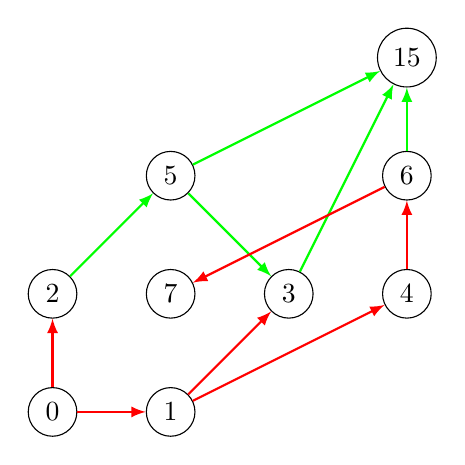
\begin{tikzpicture}
\node[draw=black,circle,minimum size=.6cm] (p0) at (0,0)  {$0$};
\node[draw=black,circle,minimum size=.6cm] (p1) at (1.5,0)  {$1$};
\node[draw=black,circle,minimum size=.6cm] (p2) at (0,1.5)  {$2$};
%\node[draw=black,circle,minimum size=.6cm] (p3) at (0,3) {};
%\node[draw=black,circle,minimum size=.6cm] (p4) at (0,4.5) {};
\node[draw=black,circle,minimum size=.6cm] (p5) at (1.5,1.5) {$7$};
\node[draw=black,circle,minimum size=.6cm] (p6) at (3,1.5) {$3$};
\node[draw=black,circle,minimum size=.6cm] (p7) at (4.5,1.5) {$4$};
\node[draw=black,circle,minimum size=.6cm] (p8) at (1.5,3) {$5$};
%\node[draw=black,circle,minimum size=.6cm] (p9) at (3,3) {};
\node[draw=black,circle,minimum size=.6cm] (p10) at (4.5,3) {$6$};
%\node[draw=black,circle,minimum size=.6cm] (p11) at (1.5,4.5) {};
%\node[draw=black,circle,minimum size=.6cm] (p12) at (3,4.5) {};
\node[draw=black,circle,minimum size=.6cm] (p13) at (4.5,4.5) {$15$};
%\node[draw=black,circle,minimum size=.6cm] (p14) at (3,0) {};
%\node[draw=black,circle,minimum size=.6cm] (p15) at  (4.5,0) {};
\draw [-latex,red,thick] (p0) edge (p1);
\draw [-latex,red,thick] (p0) edge (p2);
\draw [-latex,green,thick] (p2) edge (p8);
\draw [-latex,red,thick] (p1) edge (p6);
\draw [-latex,red,thick] (p1) edge (p7);
\draw [-latex,green,thick] (p8) edge (p13);
\draw [-latex,green,thick] (p6) edge (p13);
\draw [-latex,red,thick] (p7) edge (p10);
\draw [-latex,green,thick] (p10) edge (p13);
\draw [-latex,green,thick] (p8) edge (p6);
\draw [-latex,red,thick] (p10) edge (p5);
\end{tikzpicture}
\caption{\label{fig:1}Solvable abstract reach-avoid control problem with initial state $0$ and target state $15$. The colors of the transitions indicate two different control symbols.}
\end{figure}

\subsubsection{\texttt{test\_overapproximation}}

Some primitive intersection tests on a uniform grid in $\mathbb{R}^2$.

\section{Output files from the source code generation}

We summarize below all files created from source code generation. 
See comments of each file for more details.

\begin{center}
\renewcommand{\arraystretch}{1.2}%
\tabcolsep0pt%
\begin{tabularx}{.98\linewidth}{lp{10pt}X}
File name && Description \\
\hline
\hline
\small \texttt{dynamics\_specification\_parameters.adb} && Floating-point implementation of the user input in the Ada programming language \\
\small \texttt{dynamics\_specification\_parameters.ads} && Specification file to previous \\
\small \texttt{dynamics\_specification\_parameters.c} && Floating-point implementation of the user input in the C programming language \\
\small \texttt{dynamics\_specification\_parameters.h} && Header file to previous \\
\small\texttt{Function.adb} && Floating-point implementation of the right hand side of the unperturbed dynamics in the Ada programming language \\
\small\texttt{Function.ads} && Specification file to previous \\
\small\texttt{Function.c} && Floating-point implementation of the right hand side of the unperturbed dynamics in the C programming language \\
\small\texttt{Function.h} && Header file to previous \\
\small\texttt{Function\_ia.c} && Interval arithmetic implementation of the right hand side of the unperturbed dynamics in the C programming language  \\
\small\texttt{Function\_ia.h} && Header file to previous \\
\small\texttt{Function.mma} && Floating-point implementation of the right hand side of the unperturbed dynamics in the Mathematica programming language \\
\small\texttt{Jacobian.abcs} && Floating-point implementation of the first derivative of the right hand side of the unperturbed dynamics in the problem compiler programming language \\
\small\texttt{Jacobian.c} && Interval arithmetic implementation of the first derivative of the right hand side of the unperturbed dynamics in the C programming language \\
\small\texttt{Jacobian.h} && Header file to previous \\
\small\texttt{taylorcoefficients.abcs} && Taylor coefficients for the right hand side of the unperturbed dynamics in the problem compiler programming language \\
\small\texttt{taylorcoefficients.adb} && Taylor coefficients for the right hand side of the unperturbed dynamics in the Ada programming language \\
\small\texttt{taylorcoefficients.ads} && Specification file to previous \\
\small\texttt{taylorcoefficients.c} &&  Taylor coefficients for the right hand side of the unperturbed dynamics in the C programming language \\
\small\texttt{taylorcoefficients.h} && Header file to previous \\
\end{tabularx}
\end{center}

\noindent
Files analogous to the files listed above but for the differential
equation defining the growth bounds are contained in the subdirectory
\texttt{GrowthBounds}.
\end{document}
